\documentclass[conference]{IEEEtran}
\IEEEoverridecommandlockouts

\usepackage{cite}
\usepackage{amsmath,amssymb,amsfonts}
\usepackage{algorithmic}
\usepackage{algorithm}
\usepackage{graphicx}
\usepackage{textcomp}
\usepackage{subcaption} 
\usepackage{float}  
\usepackage{booktabs}     
\usepackage{xcolor}
\usepackage{textcomp}
\usepackage{xcolor}
\usepackage{xurl} 
\usepackage{array}
\renewcommand{\arraystretch}{1.2}
\usepackage{acronym}
% \newacro{pd}[PD]{Pierce's Disease}
\newacro{ai}[AI]{Artificial Intelligence}
\newacro{ann}[ANN]{Artificial Neural Networks}
\newacro{dl}[DL]{Deep Learning}
\newacro{ml}[ML]{Machine Learning}
\newacro{cv}[CV]{Computer Vision}
\newacro{cnn}[CNN]{Convolutional Neural Network}
\newacro{svm}[SVM]{Support Vector Machine}
\newacro{se}[SE]{Squeeze-and-Excitation}
\newacro{map}[mAP]{Mean Average Precision}
\newacro{vit}[ViT]{Vision Transormer}
\newacro{yolo}[YOLO]{You Look Only Once}
\newacro{fpn}[FPN]{Feature Pyramid Network}

\usepackage[colorlinks=true, allcolors=blue]{hyperref} 
\def\BibTeX{{\rm B\kern-.05em{\sc i\kern-.025em b}\kern-.08em
    T\kern-.1667em\lower.7ex\hbox{E}\kern-.125emX}}
\begin{document}

\title{GrapevineNet\_SE: Lightweight EfficientNet Model with SE Attention for Pierce's Disease Stage Classification}


\author{
\IEEEauthorblockN{1\textsuperscript{st} Sehrish Noreen}
\IEEEauthorblockA{\textit{Department of Software Engineering} \\
\textit{University of Sargodha}\\
Sargodha, Pakistan \\
sehrishnoreen31@gmail.com}
}

\maketitle

\begin{abstract}
Pierce's Disease is a becterial disease caused by Xylella fastidiosa. It affects the grapevine leaves. Accurate assessment of grapevine leaf health is important for precision agriculture. But traditional manual inspection is higly subjective and often inconsistent. Recent advances in \ac{dl} have enabled automated analysis of grapevine leaves. In this paper, we propose \textit{GrapevineNet\_SE}, a transfer learning model optimized for the multi-stage grapevine Pierce's Disease classification on a relatively small dataset. The model uses an EfficientNet-B0 backbone, enhanced with a \ac{se} attention module, and a compact classification head. It effectively extracts grapevine leaves feature for a better classification of disease stage. Our model achieves a training accuracy of 95.57\%, validation accuracy of 92.25\% and a test accuracy of 95.26\%, significantly outperforming baseline EfficientNet-B0 (73.07\%) and ResNet50 (65.34\%) architectures. These results highlight the model's potential to facilitate timely disease detection. It bridges the gap between baseline research models and practical precision agriculture applications.
\end{abstract}

\begin{IEEEkeywords}
Deep Learning, Computer Vision, Grapevine, Pierce Disease, EfficientNet, SE Attention
\end{IEEEkeywords}

\section{Introduction}
Pierce's Disease in grapevines is a fatal disease caused by the bacterium Xylella fastidiosa. This becterium hat lives in the xylem of grapevines. It blocks water flow and causes symptoms like leaf scorch, wilting, and eventual vine death. It spreads by insects like the Glassy-Winged Sharpshooter. Grapevine health and fruit quality are critical measures of vineyard productivity and quality. Making early disease detection and accurate assessment of leaf conditions is essential for precision viticulture. Traditionally, plant leaf disease monitoring has been done through manual inspection. Manual inspection relies completely on human observation. Different inspectors may interpret the same symptoms in different ways that leads to inconsistent conclusions about leaf health. Traditional evaluation methods do not follow any uniform standard measure. These methods are also very time consuming. Only a small part of the vineyard can be examined manually due to resource constraints.

Recent advances in \ac{cv} and \ac{dl} have transformed this domain by enabling automated analysis of grapevine leaves through high resolution images. In particular, \ac{dl} models like \ac{cnn}s, have showed greate performance in detecting and classifying morphological and spectral patterns associated with leaf health and disease/ripeness stages \cite{Zhang2024GMamba}. Existing studies highlight the efficiency of \ac{cv} approaches. \ac{cnn} classification models have achieved accuracies exceeding 95\% \cite{Sagar2025}. While hybrid architectures incorporating multi-backbone fusion or transformer modules have reported almost perfect performance near 100\% accuracy \cite{AlNasseri2025}. Object detection models, such as YOLO variants, have shown strong potential for on-field deployment of models, reaching \ac{map} up to 95\% \cite{Zhou2025YOLOGrape}. Complementary techniques including Spectroscopic Sensing and \ac{ml} approaches like \ac{svm} and Chemometric Regression have further enabled nutrient assessment and early pathogen detection with R² values up to 0.90 for macro and micronutrient prediction \cite{Manzano2025}. 

Despite these advancements, many challenges remain. Most existing models are either computationally intensive or rely on large datasets. This limits their applicability in small vineyards. Many studies focus only on binary disease detection or single-stage ripening classification. Neglecting the nuanced multi-stage progression of grapevine leaves disease. Real-time deployability and lightweight architectures suitable for edge devices are rarely addressed, leaving a gap between research and practical vineyard implementation. To address these gaps, this paper proposes \textit{GrapevineNet\_SE}, a relatively lightweight transfer learning model optimized for multi-stage grapevine leaf Pierce's Disease classification on a relatively small dataset. The model uses a frozen EfficientNet-B0 backbone with selective feature extraction. It is enhanced by a lightweight \ac{se} attention module, and a compact classification head. By fine-tuning only a subset of the EfficientNet-B0 parameters, \textit{GrapevineNet\_SE} achieves high accuracy of approximately 95\%. While  also maintained a low computational cost, making it suitable for real-time vineyard applications on edge devices.

The key contributions of this work are as follows:
\begin{itemize}
    \item A multi-stage grapevine leaf Pierce's Disease classification model.
    \item Integration of a \ac{se} attention mechanism to enhance feature representation and improve stage wise disease classification accuracy.
    \item Robust performance on training, validation, and test splits, achieving a high accuracy on all splits that indicates generalizability to unseen data.
\end{itemize}


The rest of the paper is structured as follows. Section \ref{sec:rw} reviews most recent and relevant literature on grapevine leaf disease detection, including \ac{dl} architectures, attention mechanisms, and classical machine learning approaches. Section \ref{sec:methodology} details the materials and methods, covering dataset description, preprocessing pipelines, model architecture, and training strategy. Section \ref{sec:results} presents experimental results, performance evaluation, and comparative analysis with baseline pretrained models. Finally, Section \ref{sec:con} concludes the paper with key findings, discussion of limitations, and directions for future work.


\section{Related Work}
\label{sec:rw}
Grapevine leaf disease detection has experienced significant progress over the past decade, driven by advancements in deep learning, machine learning, and spectroscopic analysis. Among these, convolutional neural networks (CNNs) have emerged as the predominant approach, owing to their superior capability in extracting spatial, textural, and morphological features from complex leaf images. For instance, \cite{Malagol2025} applied a ResNet-based architecture to quantify hair structures on grape leaves, achieving an accuracy of 95.41\%, demonstrating that CNNs can effectively capture fine-scale morphological traits. Beyond simple classification, segmentation of diseased regions has been explored to improve model interpretability and to focus on biologically relevant features. \cite{Zhang2024GMamba}, for example, employed a UNet-based state-space model on PlantVillage data, achieving an intersection-over-union (IoU) of 3.28, which highlights the potential of pixel-level disease localization for precise phenotyping. In addition, object detection methods have facilitated practical field applications by enabling automated identification of diseased areas in situ. \cite{Khan2025YOLOv7} reported a mean average precision (mAP) of 64.6\%, while a more recent YOLOv11-based approach \cite{Zhou2025YOLOGrape} significantly improved detection performance, reaching a mAP of 95.2\%.

High-performance classification has also been achieved through a wide spectrum of deep learning architectures, each offering unique advantages in accuracy, efficiency, and generalizability. ResNet variants have consistently demonstrated robust performance, as in \cite{Sagar2025}, which achieved 95\% accuracy on grape leaf datasets. Multi-backbone fusion strategies have further pushed the limits of accuracy by leveraging complementary feature representations from multiple architectures. For example, \cite{Vo2026AFCNet} combined ResNet50, EfficientNetB0, and MobileNetV2, attaining an impressive 99.83\% accuracy, showing that integrating different feature extractors can enhance classification robustness. Hybrid models that incorporate transformer-based architectures have also shown promise; \cite{Zhang2025Transformer} achieved 98.48\% accuracy, demonstrating the value of self-attention mechanisms for capturing long-range dependencies in leaf images. Similarly, cascaded CNN models, as proposed by \cite{AlNasseri2025}, approached near-perfect classification, illustrating the potential of multi-stage architectures for sequential feature refinement. Lightweight architectures optimized for computational efficiency have gained attention for edge applications. MobileNetV2 combined with Vision Transformer (ViT) modules \cite{Tanvir2025} achieved 99.2\% accuracy, while comparative evaluations \cite{Mathew2025} reported 99.5\% accuracy, highlighting the feasibility of deploying high-performing models on resource-constrained platforms. Deep convolutional neural networks (DCNNs) based on VGG16 \cite{Prasad2024} reached 99.18\% accuracy, showing that classical architectures, when carefully optimized, can still offer competitive performance. Optimized CNN models have further enhanced classification results, as evidenced by \cite{Talaat2025} achieving 99.7\% accuracy and \cite{Karim2024} reaching 99.66\%, while even simpler optimized CNN approaches \cite{Naik2025} demonstrated consistently reliable performance across multiple grape leaf disease datasets.

Beyond deep learning-based methods, classical machine learning and spectroscopic approaches provide complementary insights that are particularly valuable for nutrient assessment and early pathogen detection. Support vector machines (SVMs) combined with feature optimization, for example, were applied by \cite{Shi2025} to classify fungal spores, achieving 97.5\% accuracy, highlighting the continued relevance of traditional machine learning techniques when paired with domain-specific feature engineering. Chemometric regression models have been effectively used for predicting macro- and micronutrient concentrations, with \cite{Manzano2025} reporting an R² of 0.90 for sodium content, demonstrating the utility of spectroscopic data for vineyard nutrient monitoring. Furthermore, early detection of viral infections has been made possible through hyperspectral and multispectral sensing techniques, as shown in \cite{Lee2024}, where strong infections were identified at CT values below 35, enabling timely interventions before visible symptoms emerge.

These studies demonstrate that combining CNNs, hybrid transformers, multi-backbone fusion, and feature-based machine learning provides accurate and robust solutions for grape leaf disease detection, nutrient assessment, and pathogen monitoring. Edge-deployable models with explainable AI techniques like Grad-CAM enable practical precision viticulture, supporting rapid disease assessment, targeted treatment, and optimized vineyard management. Spectroscopic and chemometric methods complement imaging for non-destructive plant health monitoring. Overall, this convergence of techniques advances sustainable vineyard management by improving disease mitigation, nutrient optimization, and crop productivity.


\begin{figure*}[htbp]
\centerline{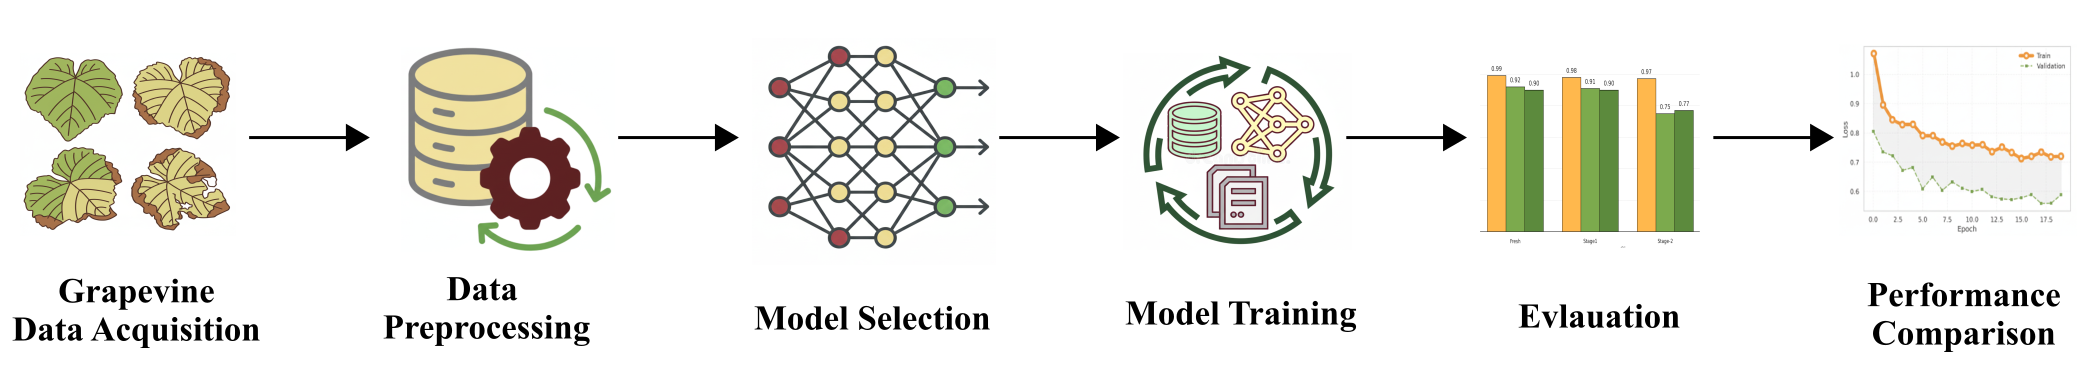
\includegraphics[width=\textwidth]{images/methodology.png}}
	\caption{Methodology}
	\label{fig:models}
\end{figure*}

\section{Material and Methods}
\label{sec:methodology}
This study implements a deep learning-based approach for detecting and classifying Pierce's Disease in grapevine leaves using convolutional neural networks. The methodology follows five sequential stages: data acquisition, preprocessing, training and evaluation, results analysis, and comparative assessment. The complete pipeline was implemented in Python using PyTorch and executed on Google Colab with GPU acceleration.

\subsection{Data Description}
The dataset comprises labeled images of grapevine leaves organized into four classes representing progressive stages of Pierce's Disease. The classification includes Fresh (healthy leaves), Stage1 (early infection), Stage-2 (moderate progression), and Stage-3 (advanced infection). Images were sourced from the GrapeVineDataSplits dataset, which provides pre-defined training, validation, and test partitions. The dataset contains 4,004 images distributed as follows: 3,203 training images, 400 validation images, and 401 test images. A consistent integer mapping was established to standardize label encoding across all subsets.

\begin{table}[h!]
    \caption{Distribution of physical images across dataset splits for grapevine Pierce's Disease stages.}
    \centering
    \begin{tabular}{m{0.2\columnwidth} m{0.2\columnwidth} m{0.2\columnwidth} m{0.2\columnwidth}}
        \toprule
        \textbf{Stage} & \textbf{Training} & \textbf{Validation} & \textbf{Test} \\
        \midrule
        Fresh   & 800 & 100 & 100 \\
        Stage 1 & 800 & 100 & 100 \\
        Stage 2 & 800 & 100 & 100 \\
        Stage 3 & 803 & 100 & 101 \\
        \midrule
        \textbf{Total} & \textbf{3203} & \textbf{400} & \textbf{401} \\
        \bottomrule
    \end{tabular}
    \label{tab:image_distribution}
\end{table}

\begin{figure}[htbp]
	\centering
    \begin{subfigure}[b]{0.24\columnwidth}
		\centering
		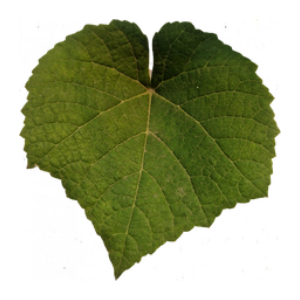
\includegraphics[width=\linewidth]{images/fresh.png} 
		\caption{Fresh Leaf}
		\label{fig:mango_sub}
	\end{subfigure}
    \begin{subfigure}[b]{0.24\columnwidth}
		\centering
		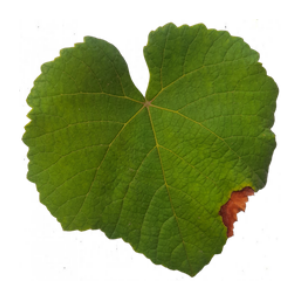
\includegraphics[width=\linewidth]{images/stage1.png} 
		\caption{Stage 1}
		\label{fig:mango_sub}
	\end{subfigure}
    \begin{subfigure}[b]{0.24\columnwidth}
		\centering
		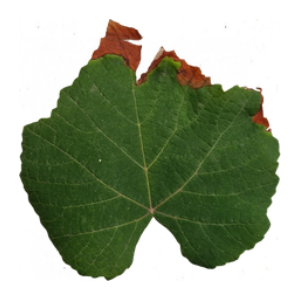
\includegraphics[width=\linewidth]{images/stage2.png} 
		\caption{Stage 2}
		\label{fig:mango_sub}
	\end{subfigure}
    \begin{subfigure}[b]{0.24\columnwidth}
		\centering
		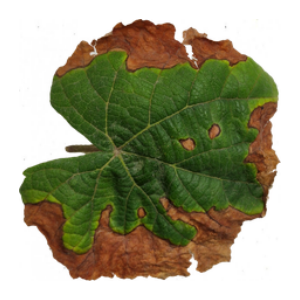
\includegraphics[width=\linewidth]{images/stage3.png} 
		\caption{Stage 3}
		\label{fig:mango_sub}
	\end{subfigure}
	\caption{Samples from Grapevine Pierce Disease dataset}
	\label{fig:objdet_sub}
\end{figure}


\subsection{Preprocessing}
Two distinct preprocessing pipelines were implemented: one for training with extensive data augmentation and another for validation/testing with minimal transformations. Training transformations included resizing to 224×224 pixels, random horizontal and vertical flipping, ±20-degree rotation, color jittering (brightness, contrast, saturation, hue adjustments), random affine transformations (translation, scaling, shearing), and ImageNet normalization. Validation and test transformations consisted only of resizing, tensor conversion, and normalization. This strategy enhances model generalization while maintaining evaluation consistency.
\begin{figure}[htbp]
\centerline{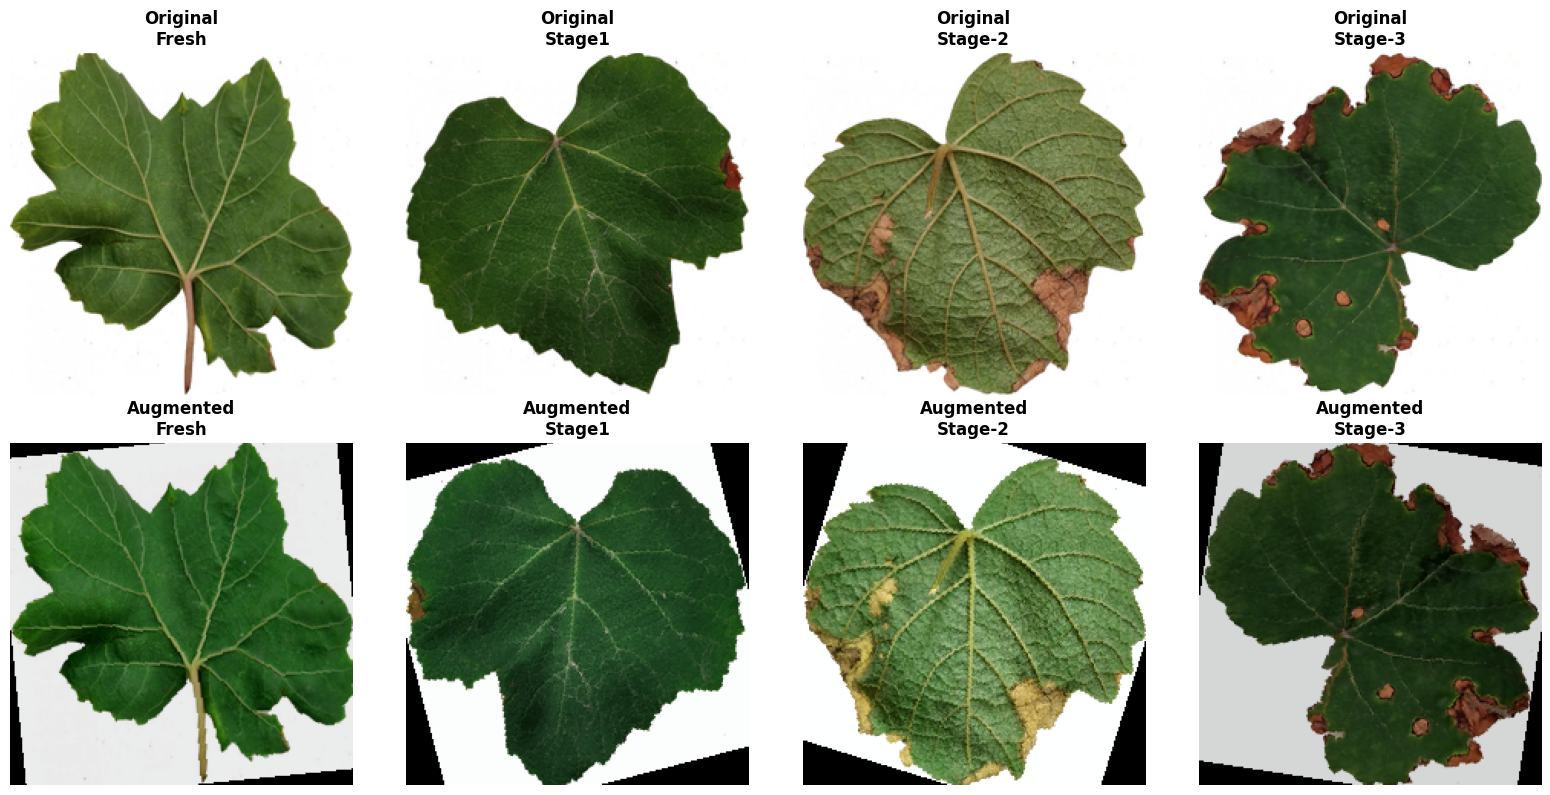
\includegraphics[width=0.9\columnwidth]{images/preprocessing.png}}
	\caption{Data preprocessing}
	\label{fig:models}
\end{figure}

\subsection{Classification and Evaluation}
The primary model, \textit{GrapevineNet\_SE}, was developed as a lightweight architecture based on EfficientNet-B0 with transfer learning.

\begin{figure*}[htbp]
\centerline{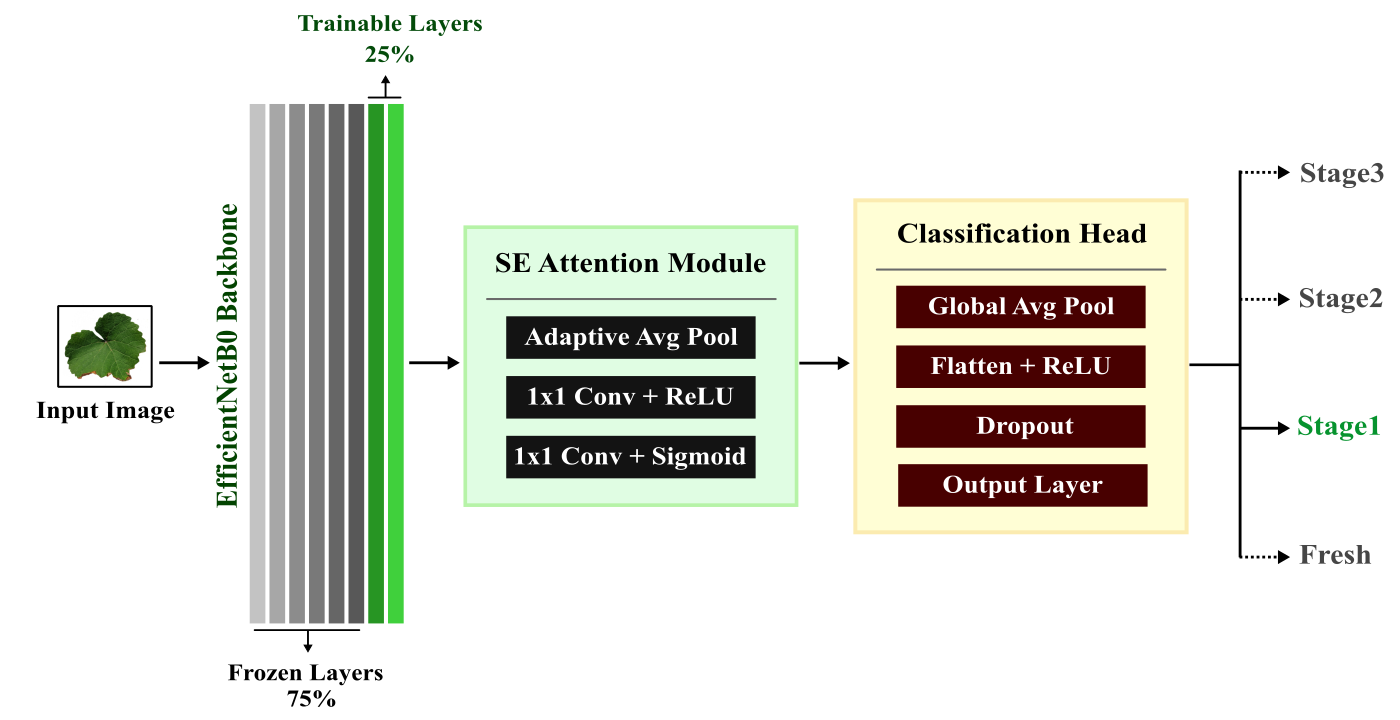
\includegraphics[width=0.9\textwidth]{images/model.png}}
	\caption{\textit{GrapevineNet\_SE} Model architecture}
	\label{fig:models}
\end{figure*}

\begin{algorithm}
\caption{GrapevineNet\_SE: Lightweight EfficientNet with SE Attention}
\label{alg:grapevinenet}
\begin{algorithmic}[1]
\STATE \textbf{Input:} Batch of grape leaf images $I$
\STATE \textbf{Output:} Predicted disease stage for each image

\STATE \textbf{Step 1: Model Setup}
\STATE Load pretrained EfficientNet-B0 backbone
\STATE Freeze first 6 blocks of \texttt{features}
\STATE Integrate SE attention module: AdaptiveAvgPool $\rightarrow$ Conv2d $\rightarrow$ ReLU $\rightarrow$ Conv2d $\rightarrow$ Sigmoid
\STATE Add classification head: AdaptiveAvgPool $\rightarrow$ Flatten $\rightarrow$ Linear(1280,512) $\rightarrow$ ReLU $\rightarrow$ Dropout $\rightarrow$ Linear(512,4)

\STATE \textbf{Step 2: Forward Pass}
\FOR{each batch of images}
    \STATE Extract features: $x \gets \texttt{backbone.features}(I)$
    \STATE Apply SE attention: $x \gets \texttt{SE}(x) * x$
    \STATE Compute predictions: $y \gets \texttt{classifier}(x)$
\ENDFOR

\STATE \textbf{Step 3: Training and Optimization}
\STATE Compute cross-entropy loss
\STATE Update unfrozen parameters using optimizer (e.g., AdamW)
\STATE Apply learning rate scheduling and early stopping based on validation performance

\STATE \textbf{Step 4: Evaluation}
\STATE Evaluate on validation set and return trained model
\end{algorithmic}
\end{algorithm}


Approximately 75\% of early backbone layers were frozen to preserve pretrained feature representations. A Squeeze-and-Excitation attention module was integrated to enhance discriminative feature learning, followed by a custom classification head with dropout regularization. Training employed AdamW optimizer with differential learning rates (backbone: 1e-4, classifier: 1e-3), cross-entropy loss with label smoothing, OneCycleLR scheduler with cosine annealing, mixed precision training, and early stopping after five epochs without validation improvement. For benchmarking, standard EfficientNet-B0 and ResNet50 architectures were implemented under identical training conditions.

\subsubsection{Evaluation Metrics}
Model performance was quantitatively assessed using standard classification metrics computed from the confusion matrix. The macro-averaging approach was employed to give equal weight to all classes regardless of sample distribution.

\begin{itemize}
    \item \textbf{Accuracy}: Macro-averaged proportion of correctly classified samples:
    \begin{equation}
        \text{Accuracy} = \frac{1}{N} \sum_{i=1}^{N} \frac{TP_i + TN_i}{TP_i + TN_i + FP_i + FN_i}
    \end{equation}

    \item \textbf{Precision}: Macro-averaged ratio of true positive predictions to all positive predictions for each class:
    \begin{equation}
        \text{Precision} = \frac{1}{N} \sum_{i=1}^{N} \frac{TP_i}{TP_i + FP_i}
    \end{equation}

    \item \textbf{Recall}: Macro-averaged ratio of true positive predictions to all actual positive samples:
    \begin{equation}
        \text{Recall} = \frac{1}{N} \sum_{i=1}^{N} \frac{TP_i}{TP_i + FN_i}
    \end{equation}

    \item \textbf{F1-Score}: Harmonic mean of precision and recall, macro-averaged:
    \begin{equation}
        \text{F1-Score} = \frac{1}{N} \sum_{i=1}^{N} \frac{2 \cdot \text{Precision}_i \cdot \text{Recall}_i}{\text{Precision}_i + \text{Recall}_i}
    \end{equation}
\end{itemize}

Confusion matrices were visualized to analyze misclassification patterns, and per-class classification reports were generated to provide detailed performance across all disease stages.


\section{Results and Discussion}
\textit{GrapevineNet\_SE} achieved superior performance across all evaluation metrics. On the test set, the model attained 95.26\% accuracy, with comparable precision, recall, and F1-scores.

\begin{figure}[htbp]
\centerline{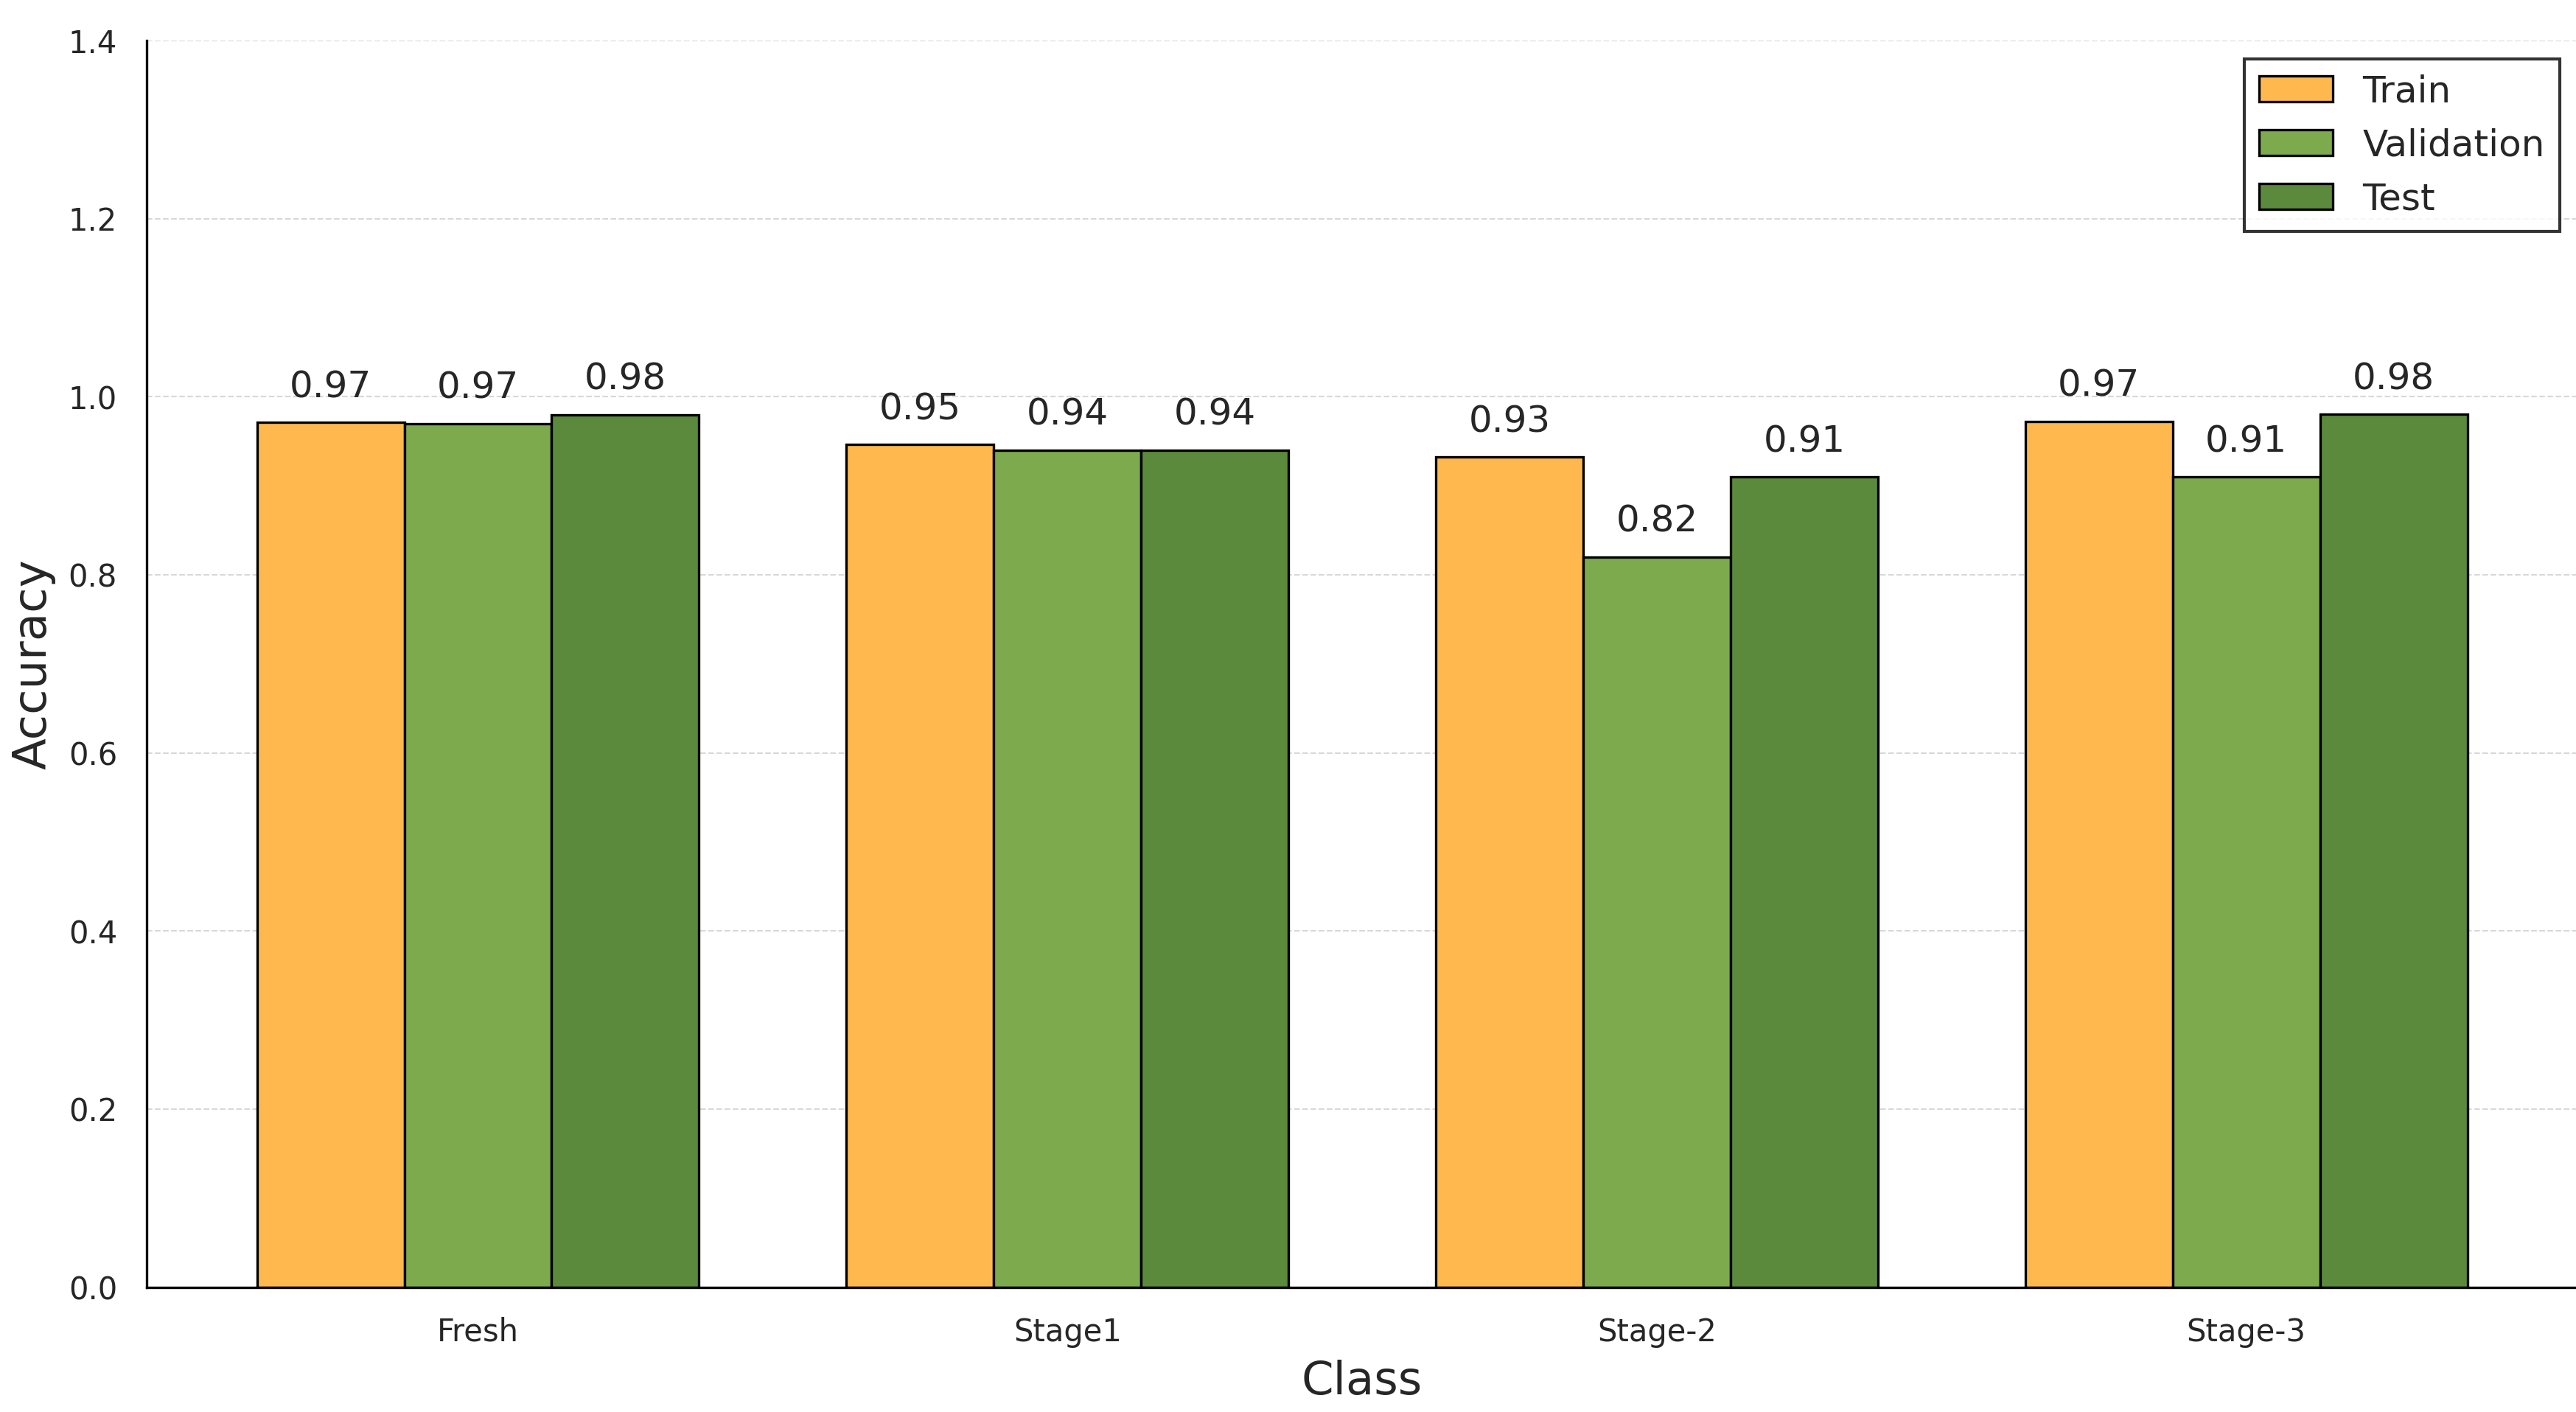
\includegraphics[width=0.9\columnwidth]{images/per_class_accuracy_all_sets.png}}
	\caption{\textit{GrapevineNet\_SE} Per class accuracies}
	\label{fig:models}
\end{figure}

\begin{figure*}[htbp]
	\centering
    \begin{subfigure}[b]{0.24\textwidth}
		\centering
		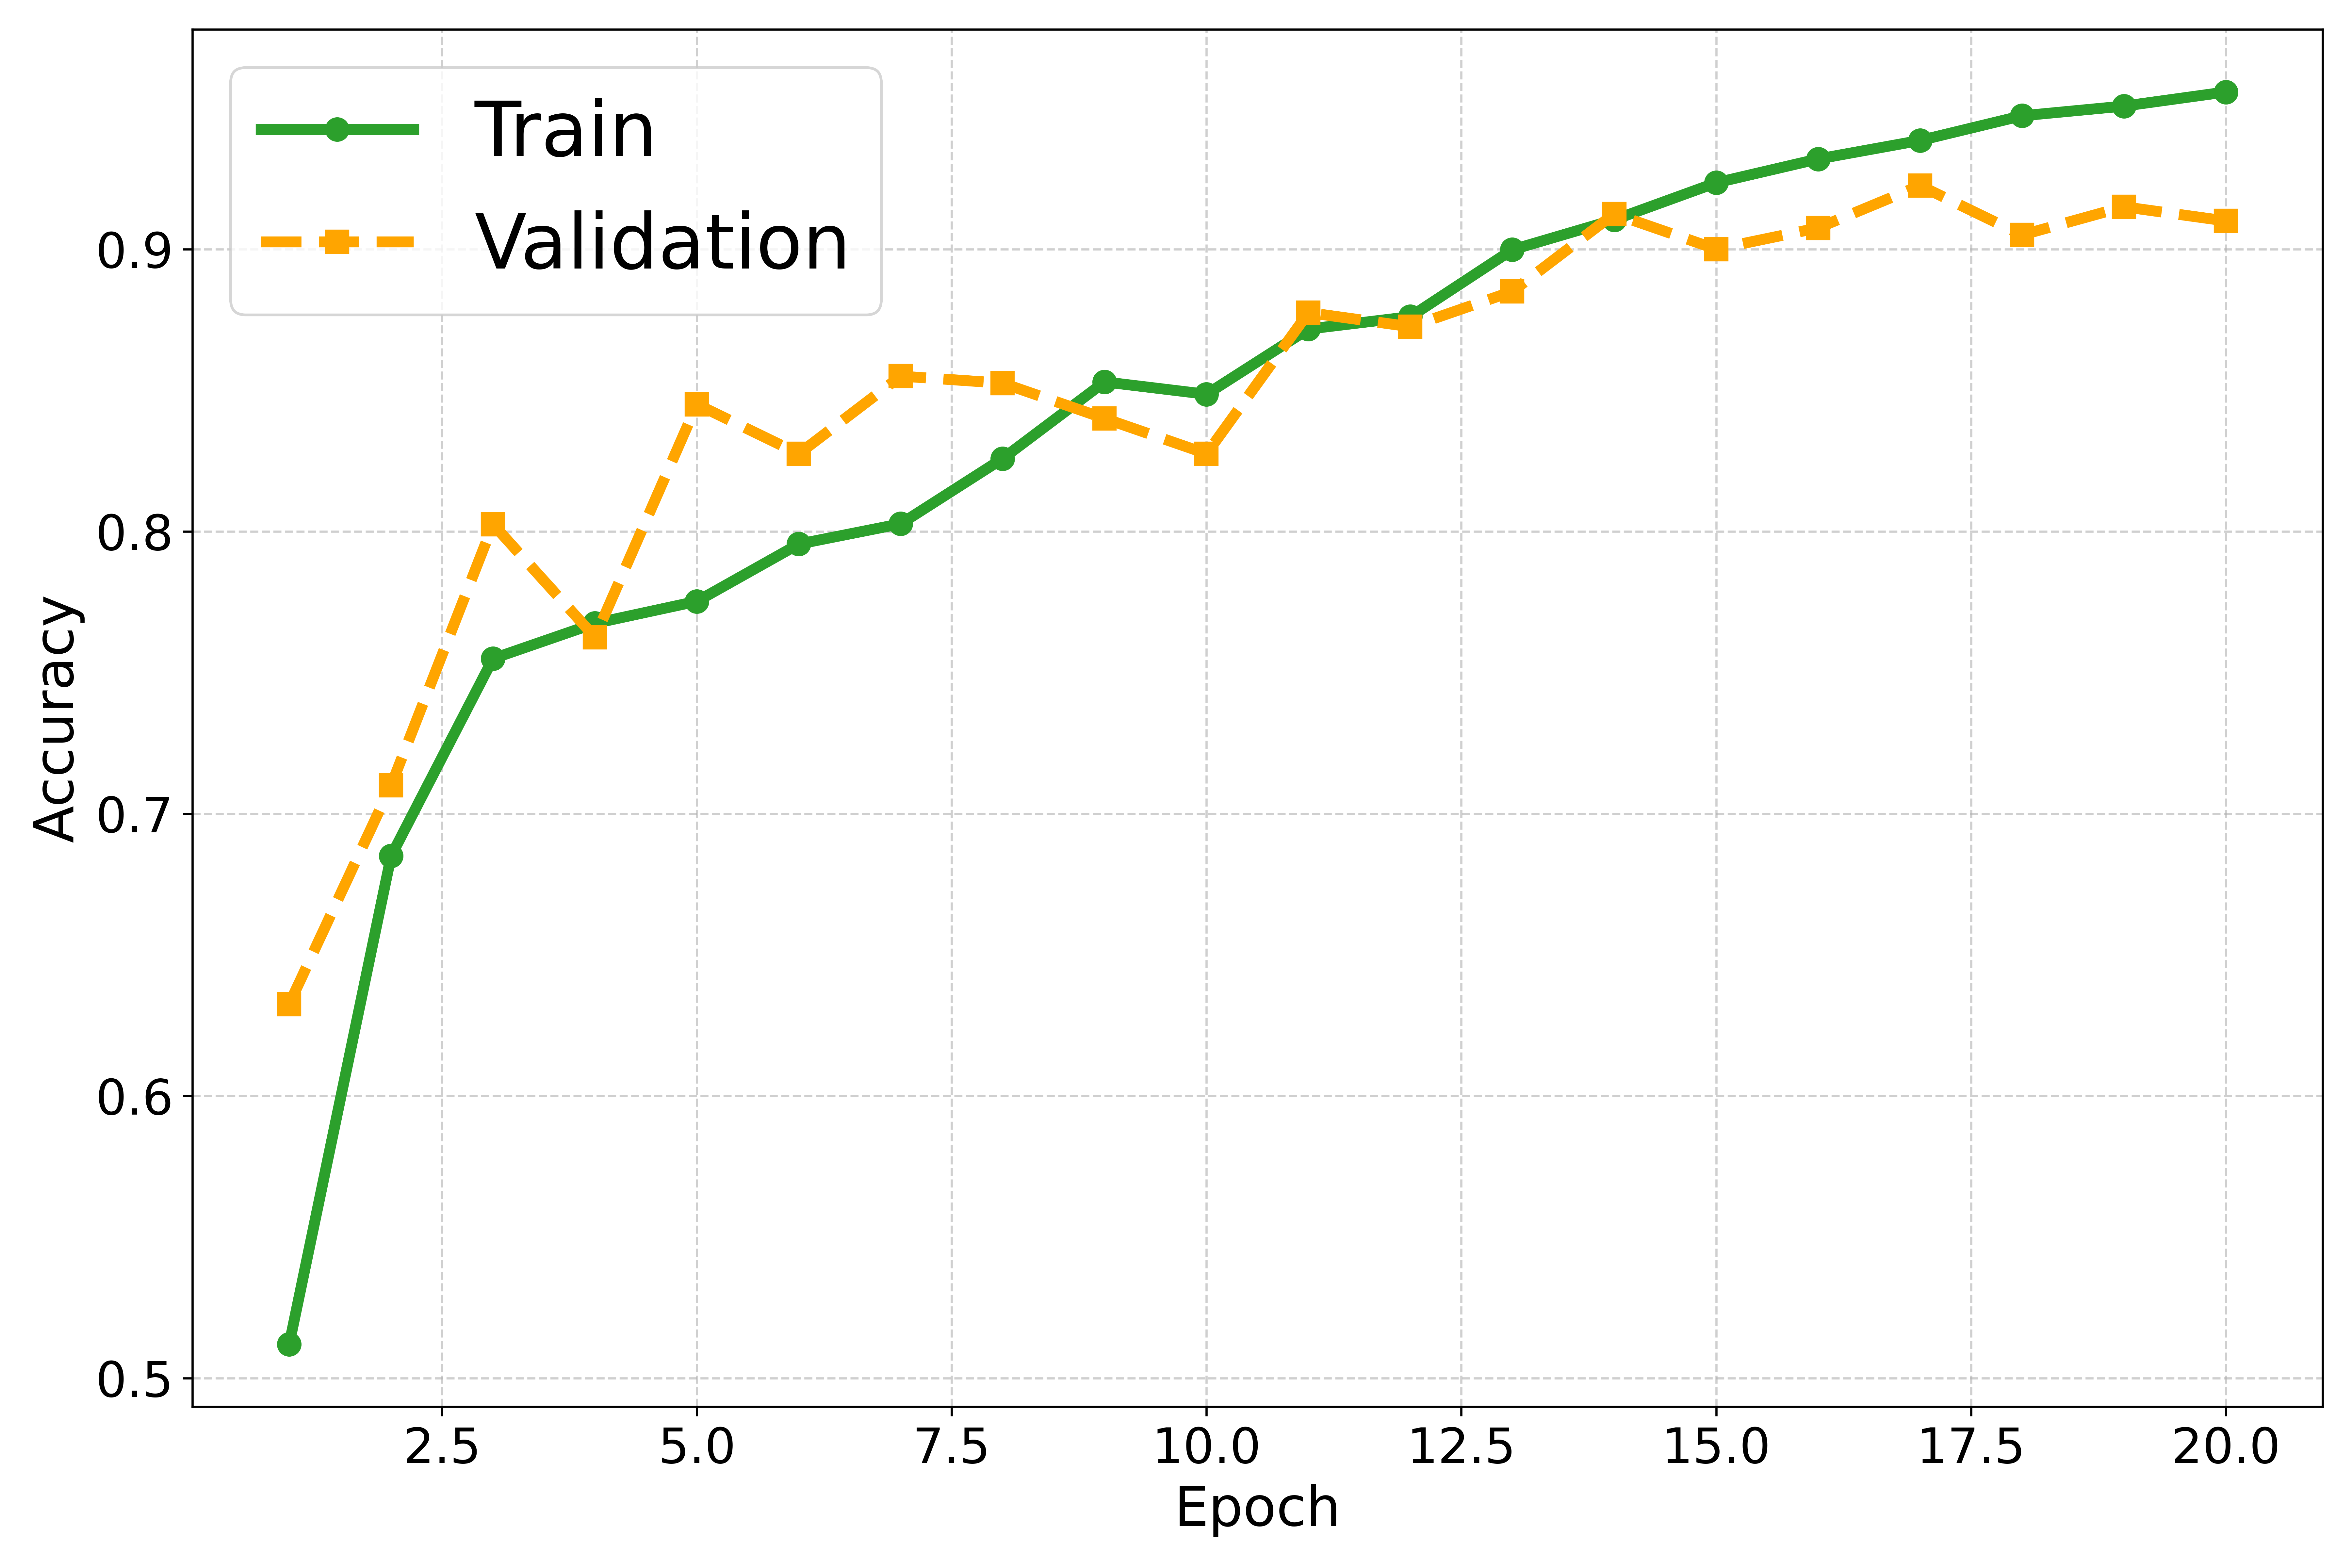
\includegraphics[width=\linewidth]{images/accuracy_plot.png} 
		\caption{Accuracy}
		\label{fig:mango_sub}
	\end{subfigure}
	\begin{subfigure}[b]{0.24\textwidth}
		\centering
		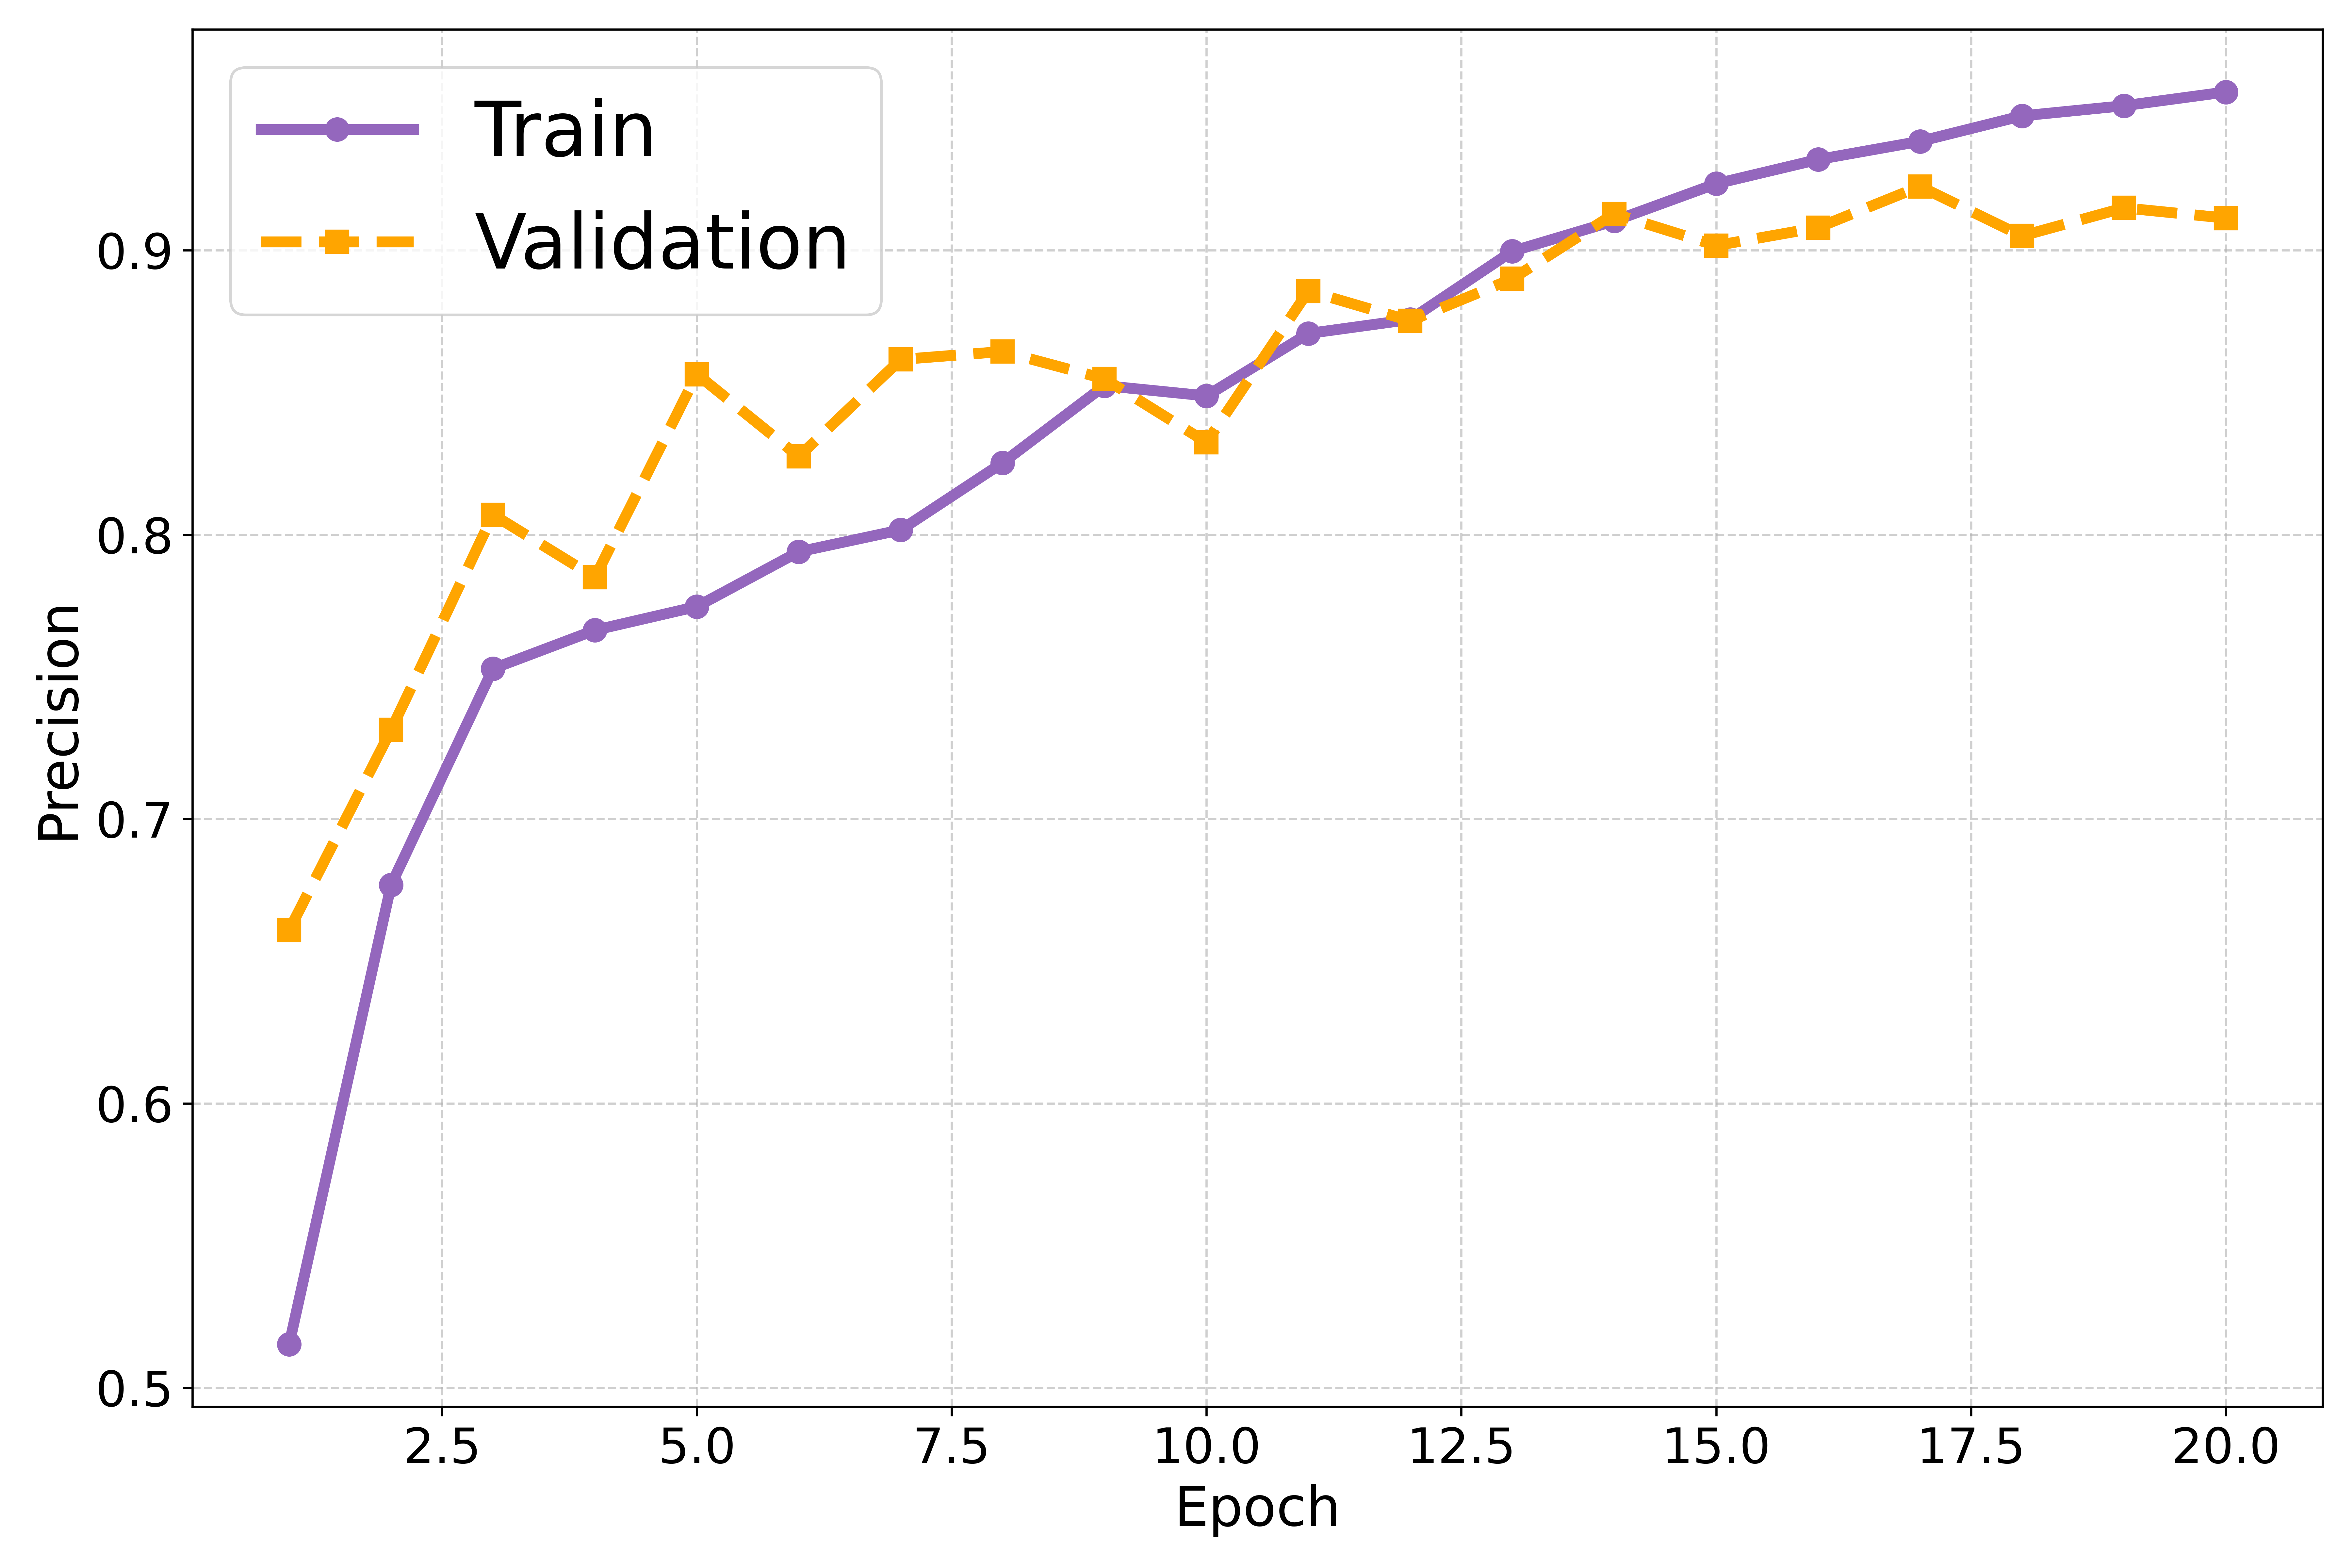
\includegraphics[width=\linewidth]{images/precision_plot.png} 
		\caption{Precision}
		\label{fig:annot_sub}
	\end{subfigure}
    \begin{subfigure}[b]{0.24\textwidth}
		\centering
		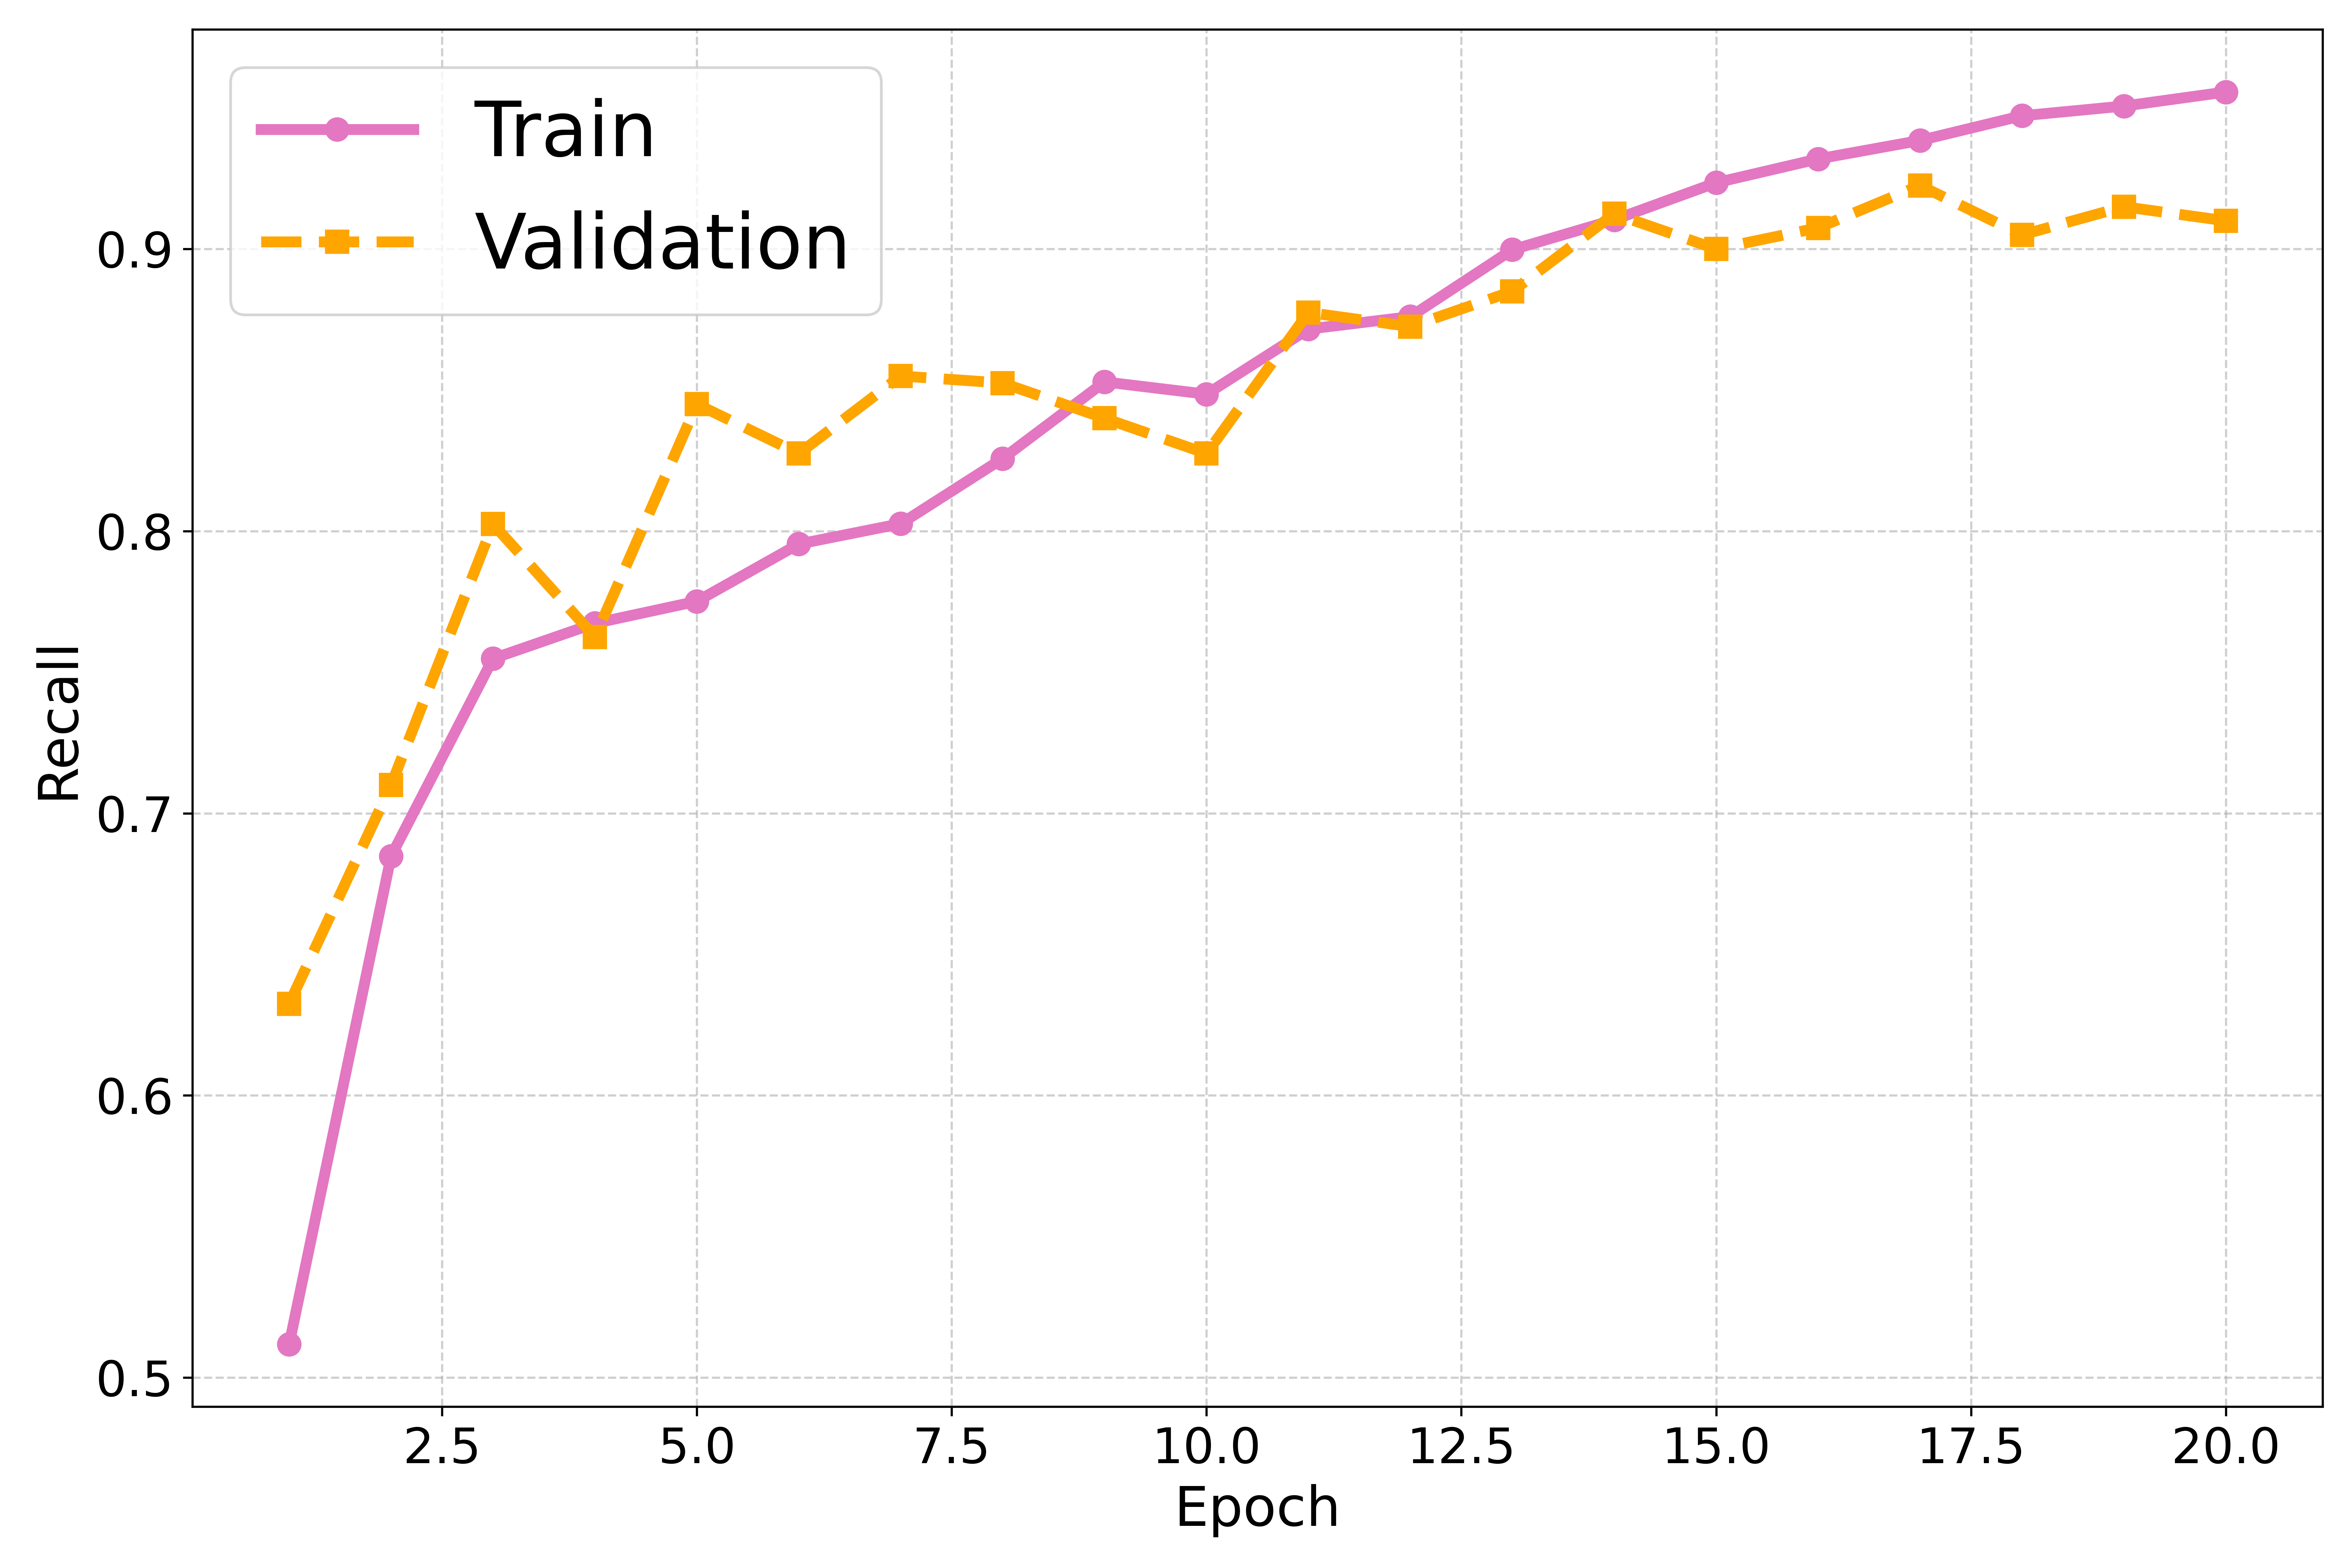
\includegraphics[width=\linewidth]{images/recall_plot.png} 
		\caption{Recall}
		\label{fig:mango_sub}
	\end{subfigure}
    \begin{subfigure}[b]{0.24\textwidth}
		\centering
		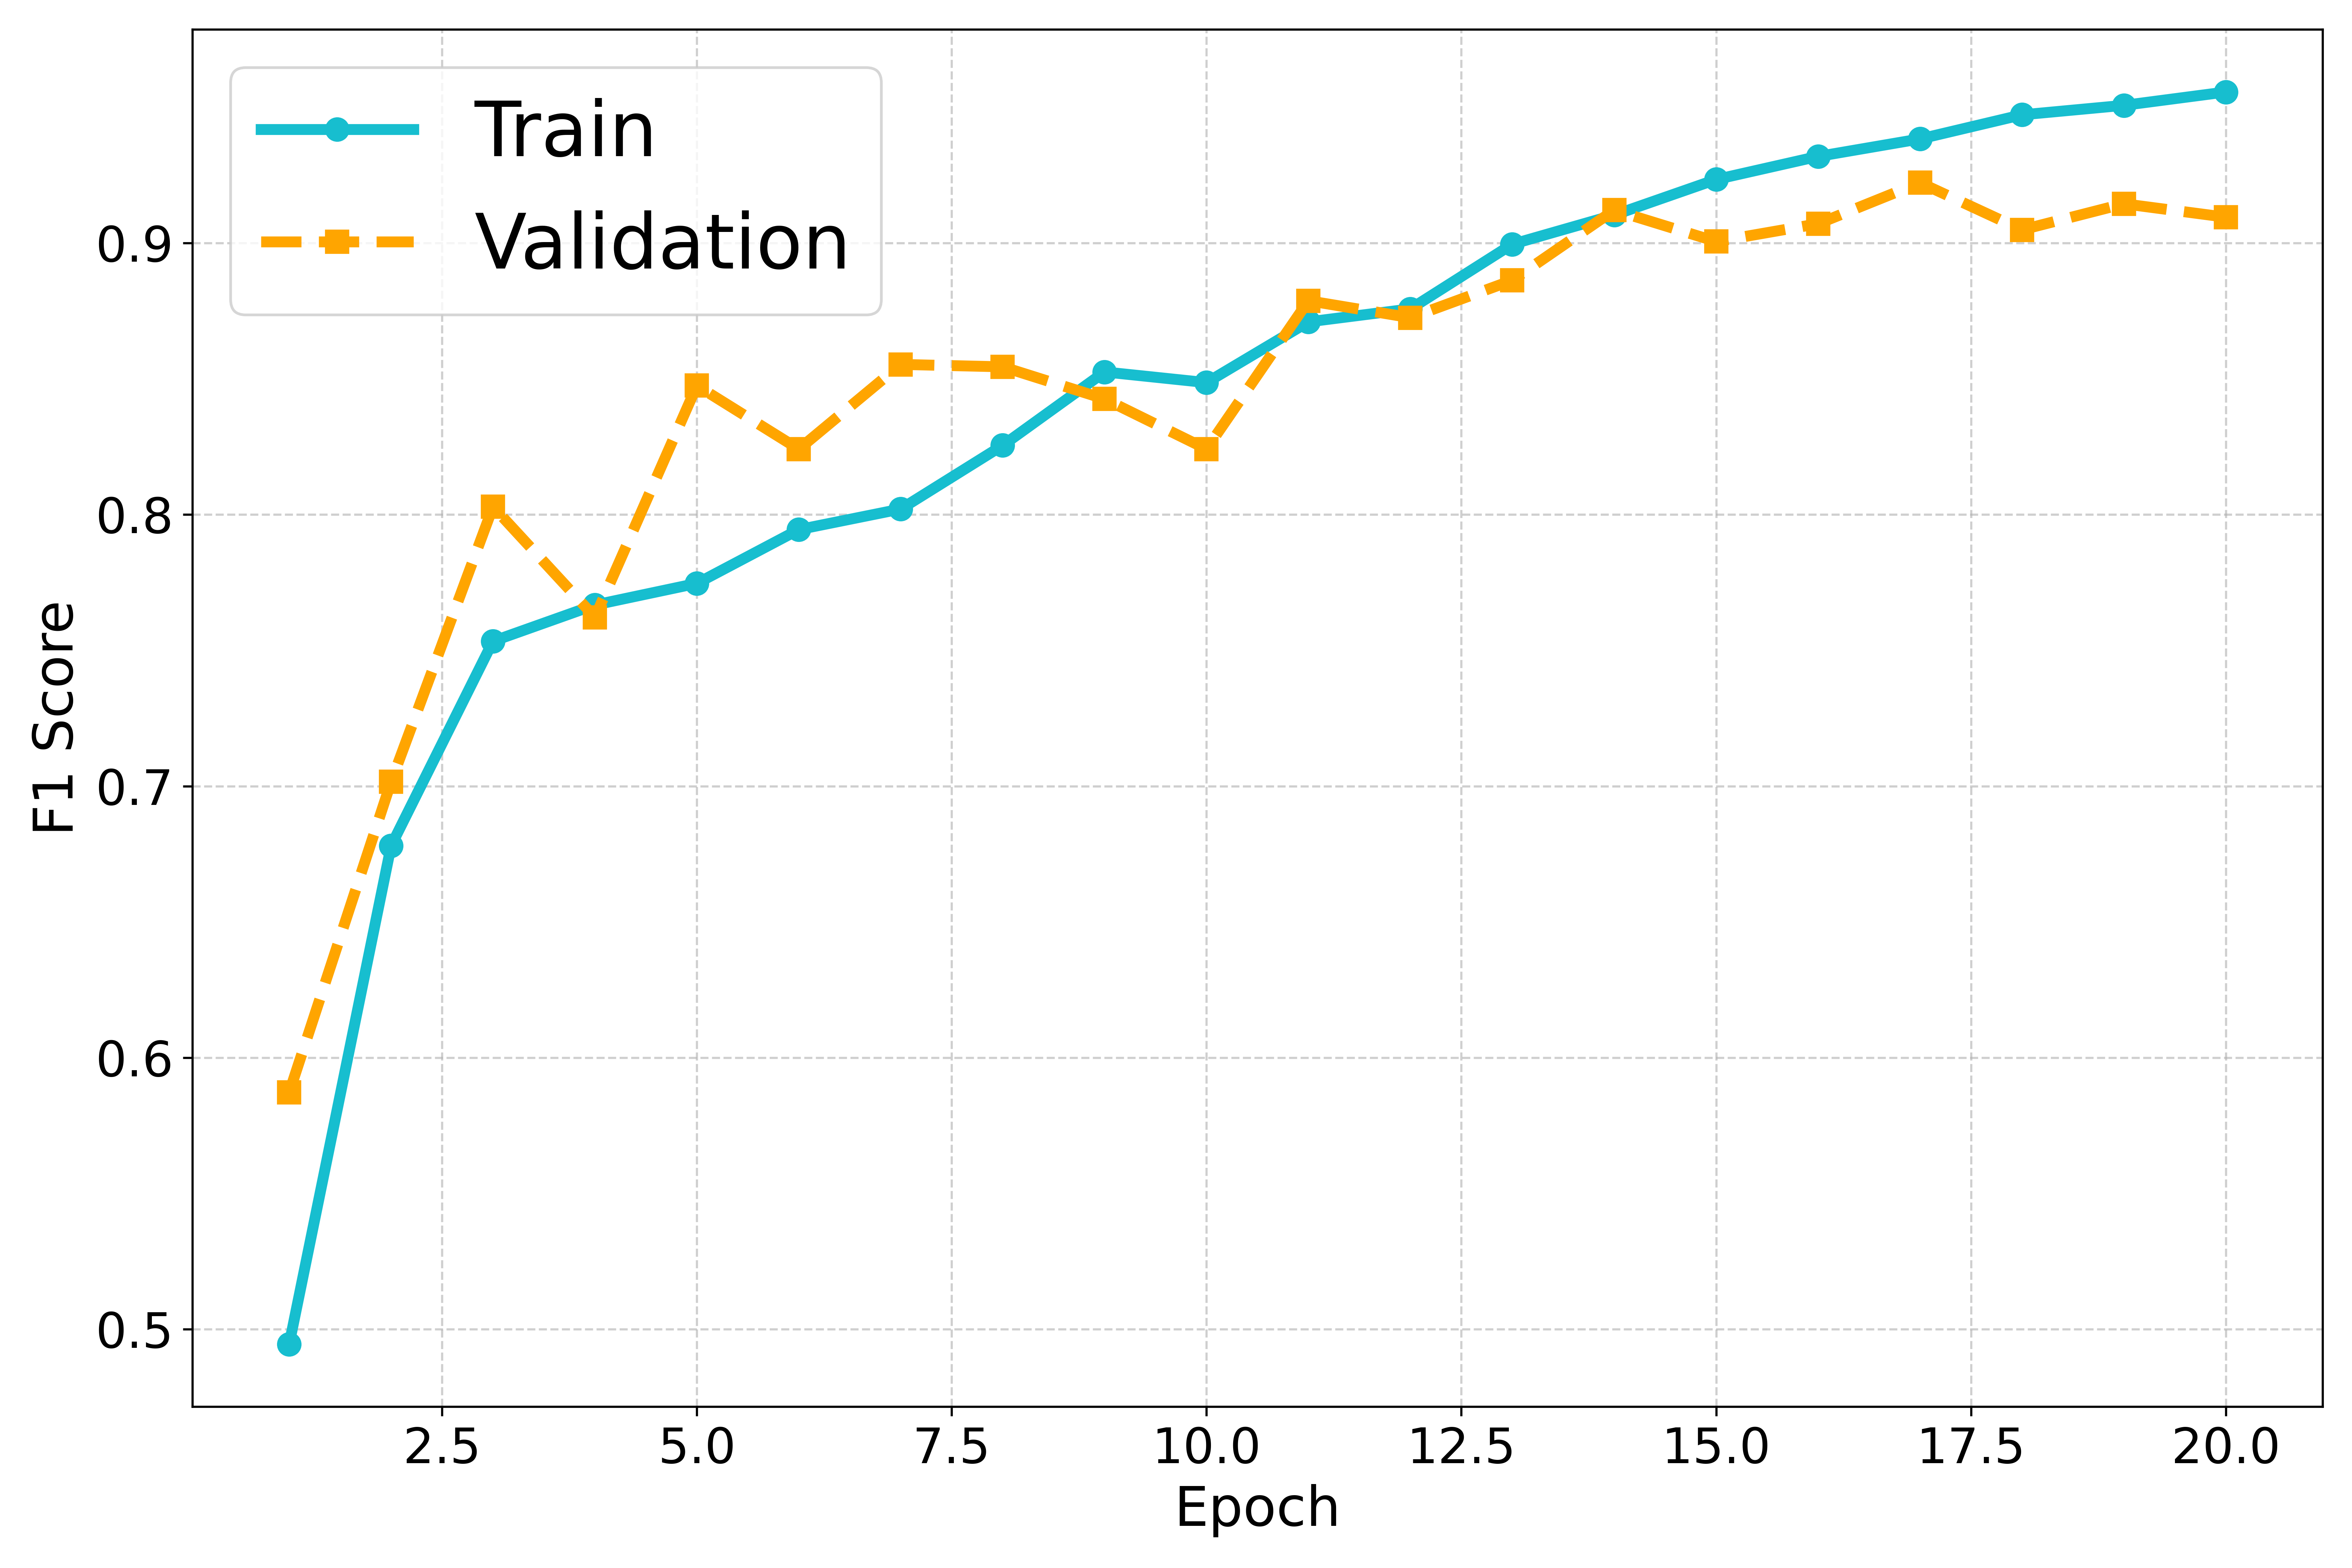
\includegraphics[width=\linewidth]{images/f1_plot.png} 
		\caption{F1-Score}
		\label{fig:mango_sub}
	\end{subfigure}
	\caption{\textit{GrapevineNet\_SE} Metrics}
	\label{fig:objdet_sub}
\end{figure*}


\begin{figure}[htbp]
\centerline{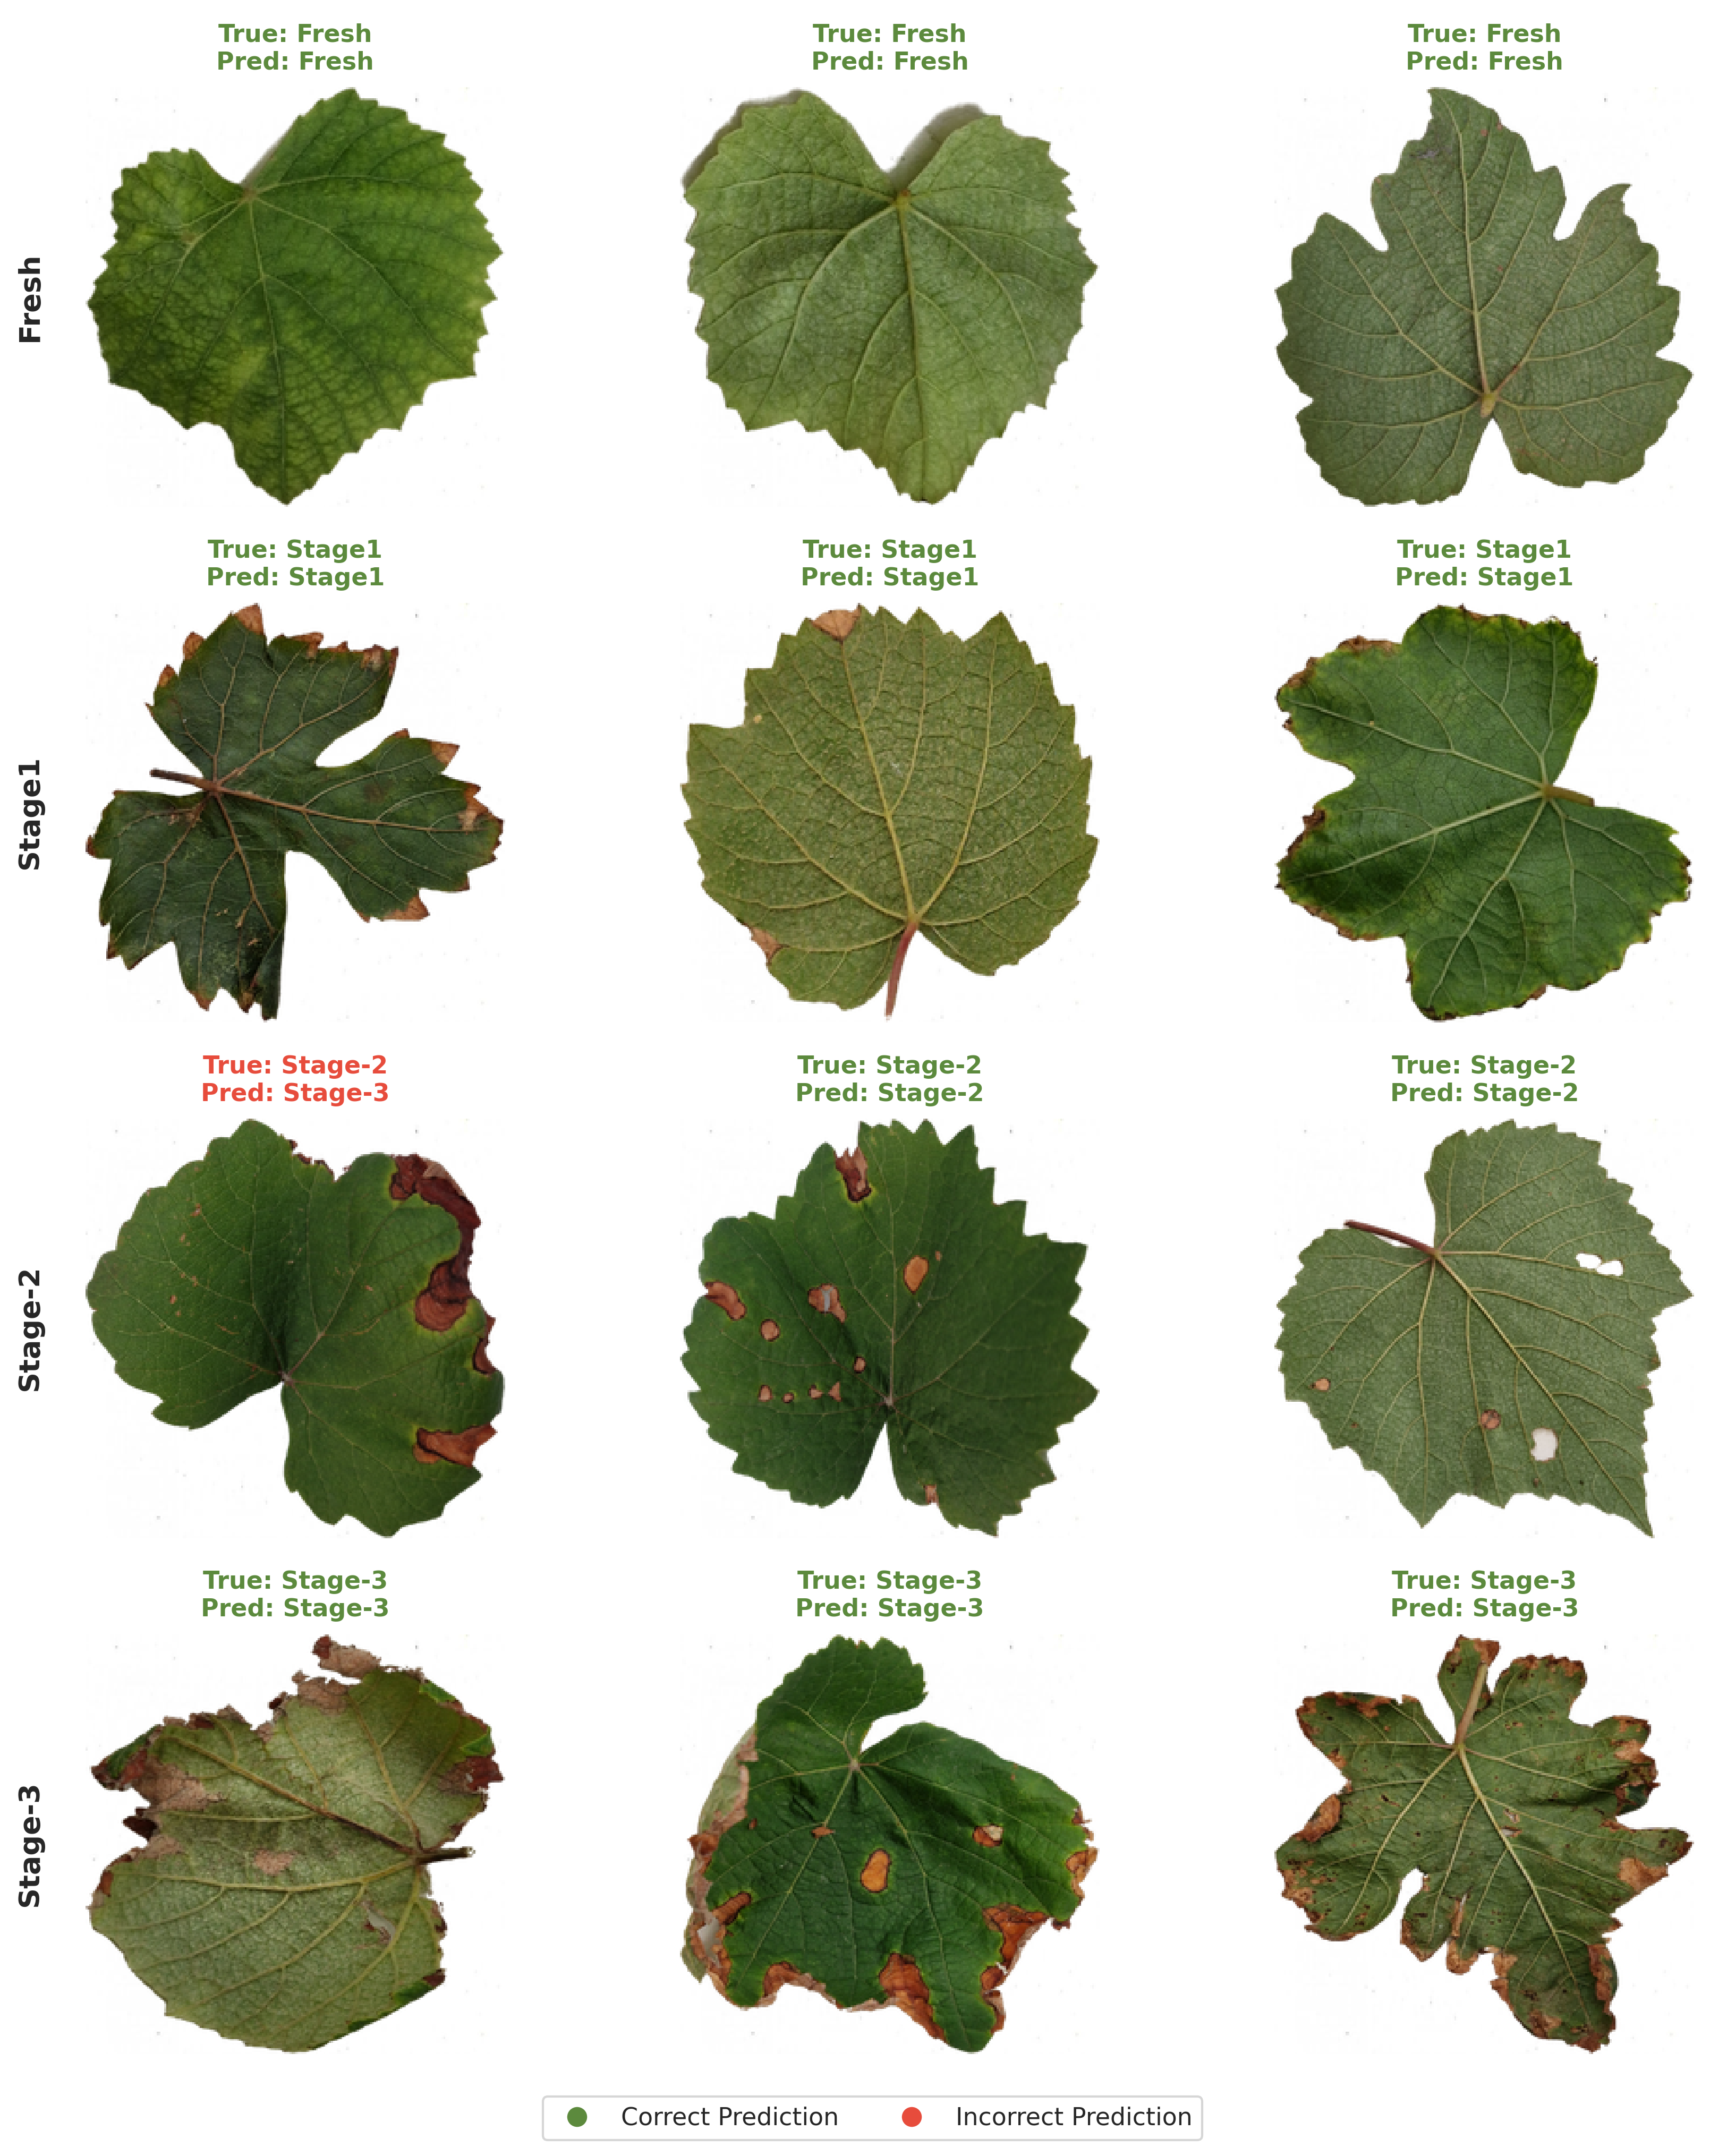
\includegraphics[width=\columnwidth]{images/test_samples_visualization.png}}
	\caption{\textit{GrapevineNet\_SE} Model prediction samples for test data}
	\label{fig:models}
\end{figure}
The confusion matrix revealed that most misclassifications occurred between adjacent disease stages, indicating logical progression in severity classification rather than random errors. Model convergence showed consistent improvement throughout training, with validation accuracy reaching 92.25\% at the best epoch and test performance exceeding both baseline architectures.

\begin{figure}[htbp]
\centerline{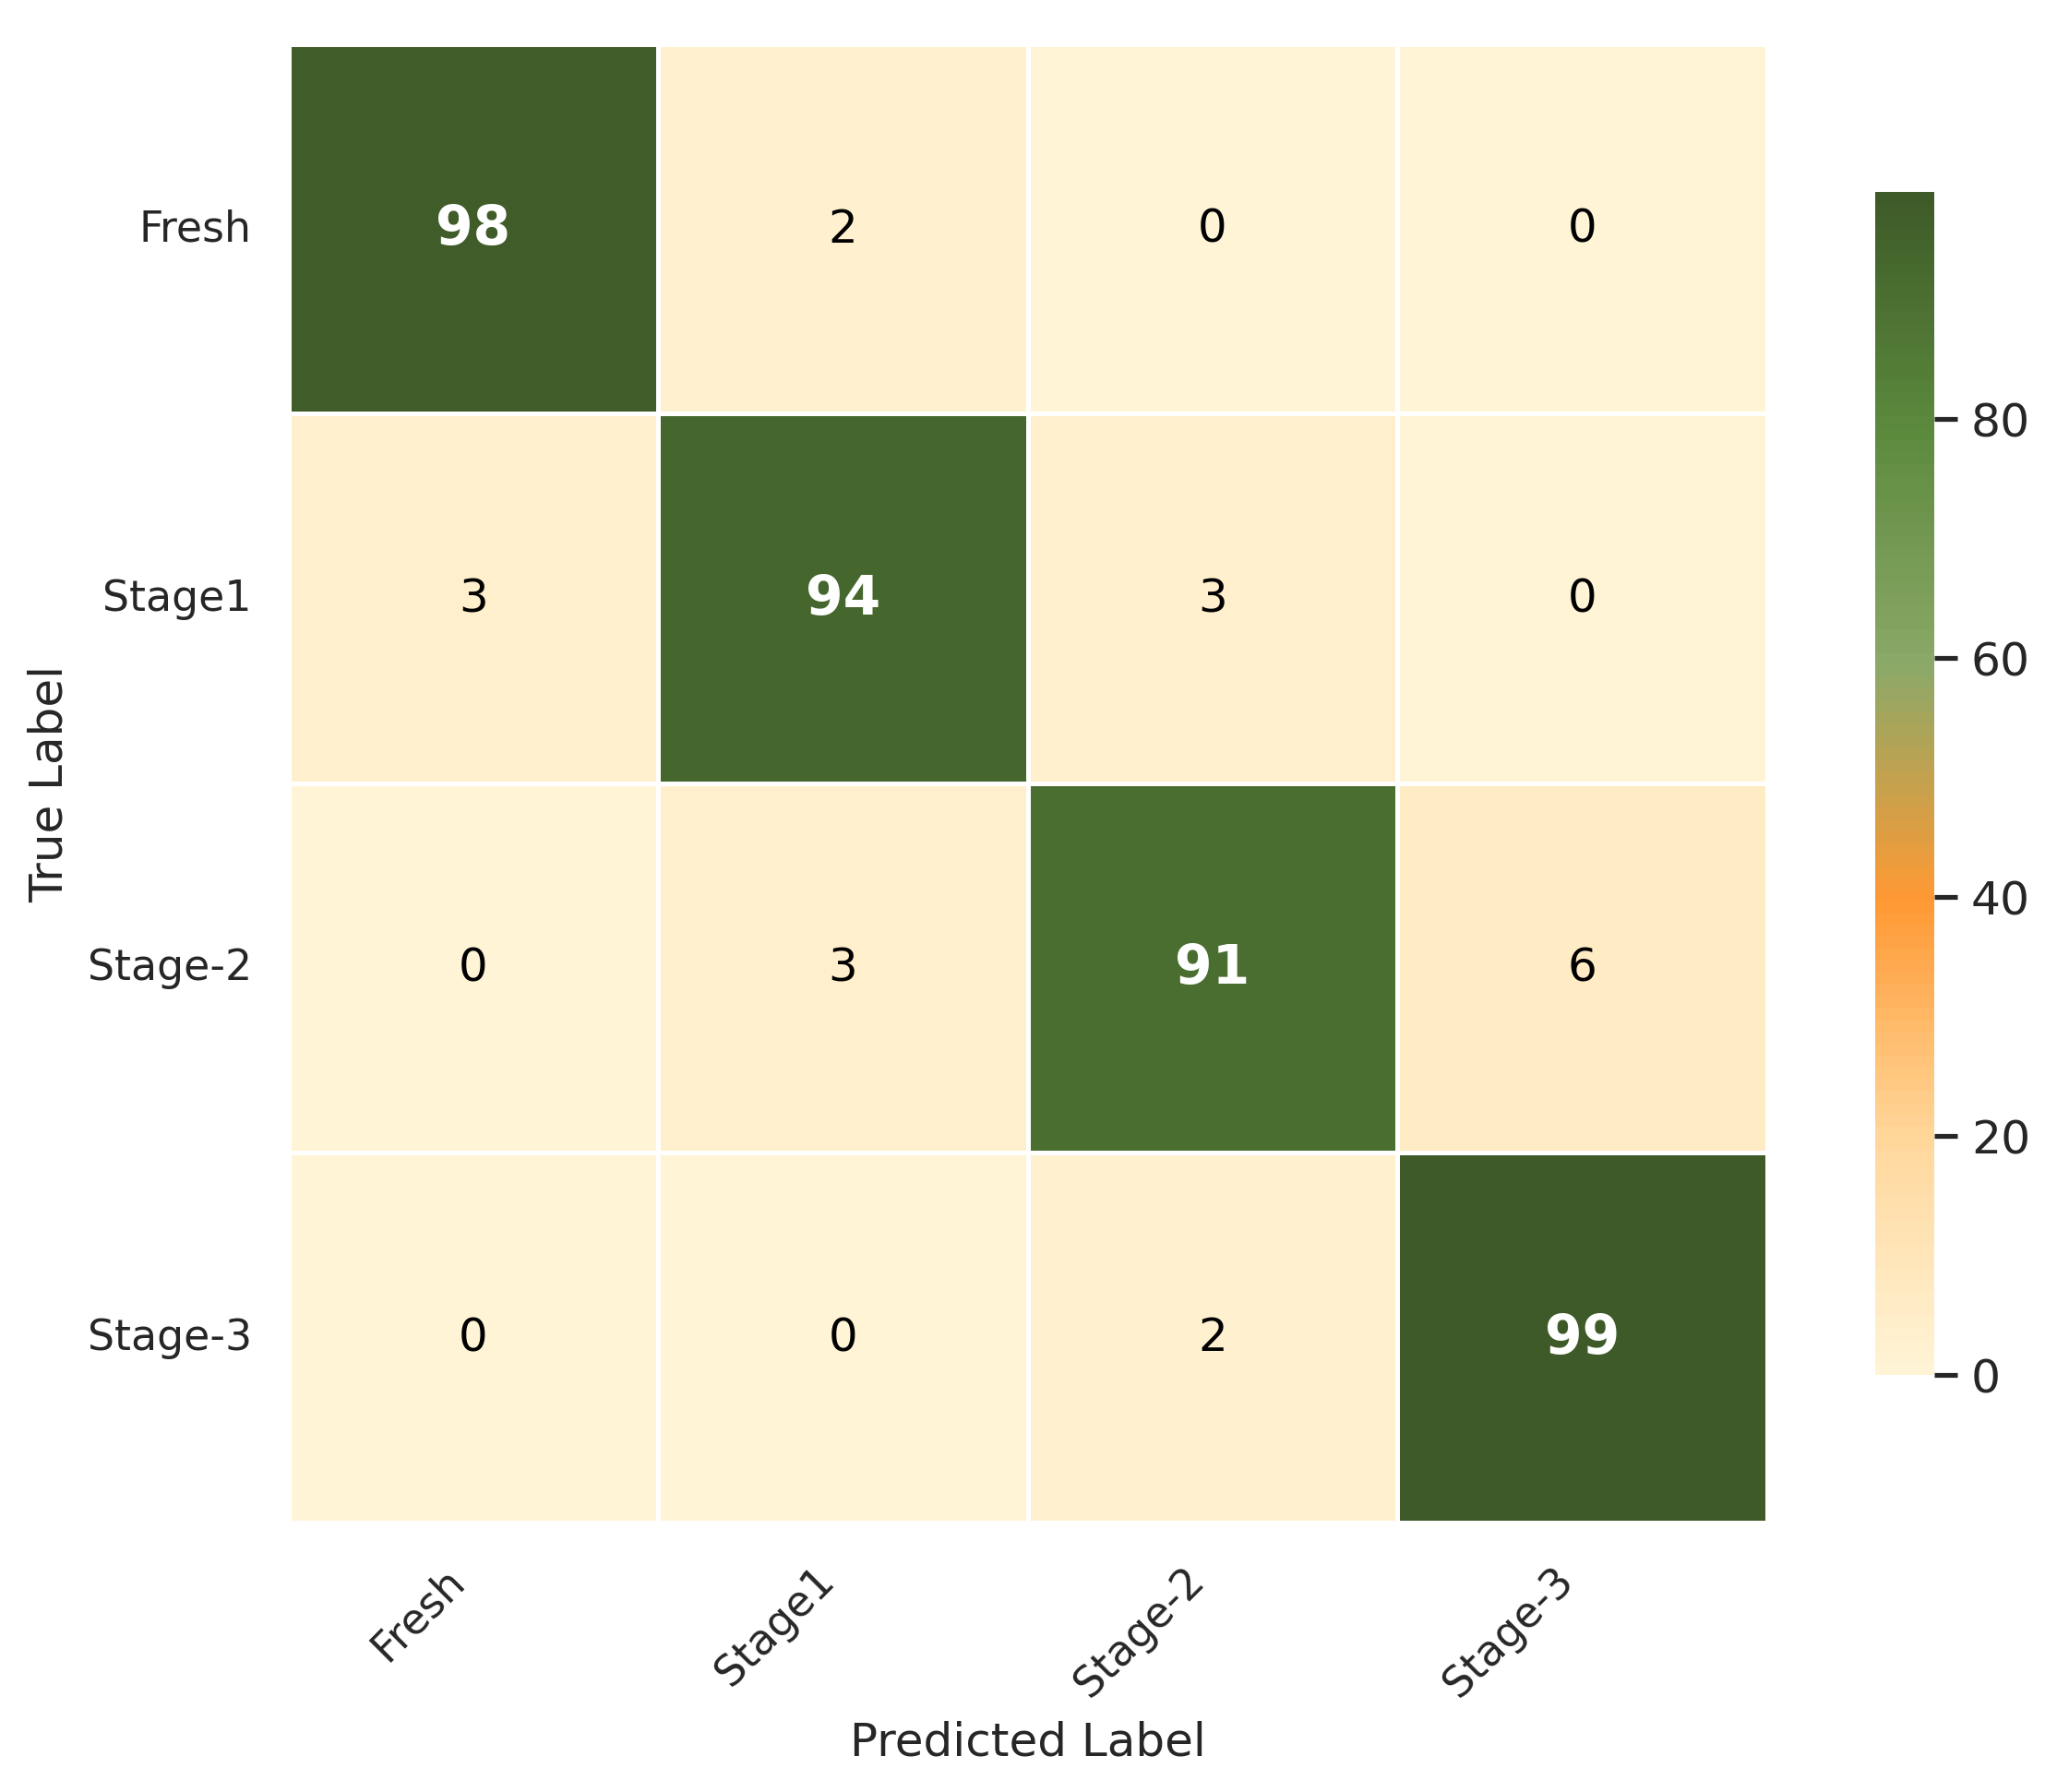
\includegraphics[width=0.7\columnwidth]{images/confusion_matrix_test.png}}
	\caption{\textit{GrapevineNet\_SE} Confusion Matrix for test data}
	\label{fig:models}
\end{figure}


\section{Comparison and Analysis}
Comparative analysis against standard EfficientNet-B0 and ResNet50 architectures demonstrated the effectiveness of the proposed model modifications. The baseline EfficientNet-B0 achieved 73.07\% accuracy while ResNet50 reached 65.34\% on the test set, both significantly lower than \textit{GrapevineNet\_SE}'s 95.26\%. This performance improvement can be attributed to the strategic layer freezing, attention mechanisms, and optimized classification head design. The results indicate that carefully designed lightweight architectures with attention modules can outperform standard pretrained models for domain-specific agricultural disease detection tasks.

\begin{table}[h!]
\caption{Comparison of \textit{GrapevineNet\_SE} with Pretrained Models on Test Set}
\centering
\begin{tabular}{m{0.23\columnwidth} m{0.09\columnwidth} m{0.09\columnwidth} m{0.09\columnwidth} m{0.09\columnwidth} m{0.09\columnwidth} m{0.09\columnwidth}}
\toprule
\textbf{Model} & \textbf{Accuracy} & \textbf{Precision} & \textbf{Recall} & \textbf{F1} & \textbf{Params (M)} \\
\midrule
\textbf{\textit{GrapevineNet\_SE}} & \textbf{0.9526} & \textbf{0.9526} & \textbf{0.9525} & \textbf{0.9524} & \textbf{4.87} \\
EfficientNet-B0 & 0.7307 & 0.7290 & 0.7307 & 0.7261 & 5.3 \\
ResNet50 & 0.6534 & 0.6816 & 0.6534 & 0.6563 & 25.6  \\
\bottomrule
\end{tabular}
\label{tab:model_comparison}
\end{table}


\section{Conclusion}
\label{sec:con}
TIn this paper, we developed a lightweight and efficient model for multi-stage classification of grapevine leaves affected by Pierce disease. The combination of a frozen EfficientNet-B0 backbone, SE attention module, and compact classification head enabled high accuracy while keeping computational costs low. Analysis of misclassifications showed that errors were primarily between adjacent stages, indicating the model captures disease progression effectively. Overall, the model provides a practical solution for real-time vineyard monitoring, supporting early disease detection and precision viticulture. Future work will focus on in-field deployment and extension to other grapevine diseases.

\vspace{12pt}
\color{black}

\bibliographystyle{IEEEtran}
\bibliography{references}
\end{document}